% ============================================================================
% Chapter 5: Implementation
% Thesis: Fuzzy Margin Representation Learning for Explainable
%         Architecture–Genotype Associations in Lung Adenocarcinoma
%         under Data Scarcity
% Author: Servio F. Lima
% University of Fribourg
% ============================================================================

\chapter{Implementation}
\label{ch:implementation}

This chapter describes the concrete software realisation of the three computational artifacts and the integrative LCHAI system designed in Chapter~\ref{ch:methodology}.
Following the Design Science Research principle of separating artifact construction from evaluation, this chapter focuses on \emph{how} each component was built: the hardware and software environment, the data acquisition and preprocessing pipelines, the neural network implementations, and the integrative clinical decision support prototype.
The evaluation of these artifacts is deferred to Chapter~\ref{ch:evaluation}.

The implementation is organised around the three-stage pipeline illustrated in Figure~\ref{fig:implementation_pipeline}: data acquisition (Section~\ref{sec:impl:data}), pattern classification (Section~\ref{sec:impl:pattern}), and mutation prediction (Section~\ref{sec:impl:mutation}).
Section~\ref{sec:impl:lchai} presents the LCHAI system prototype, and Section~\ref{sec:impl:reproducibility} addresses reproducibility.

\begin{figure}[ht!]
    \centering
    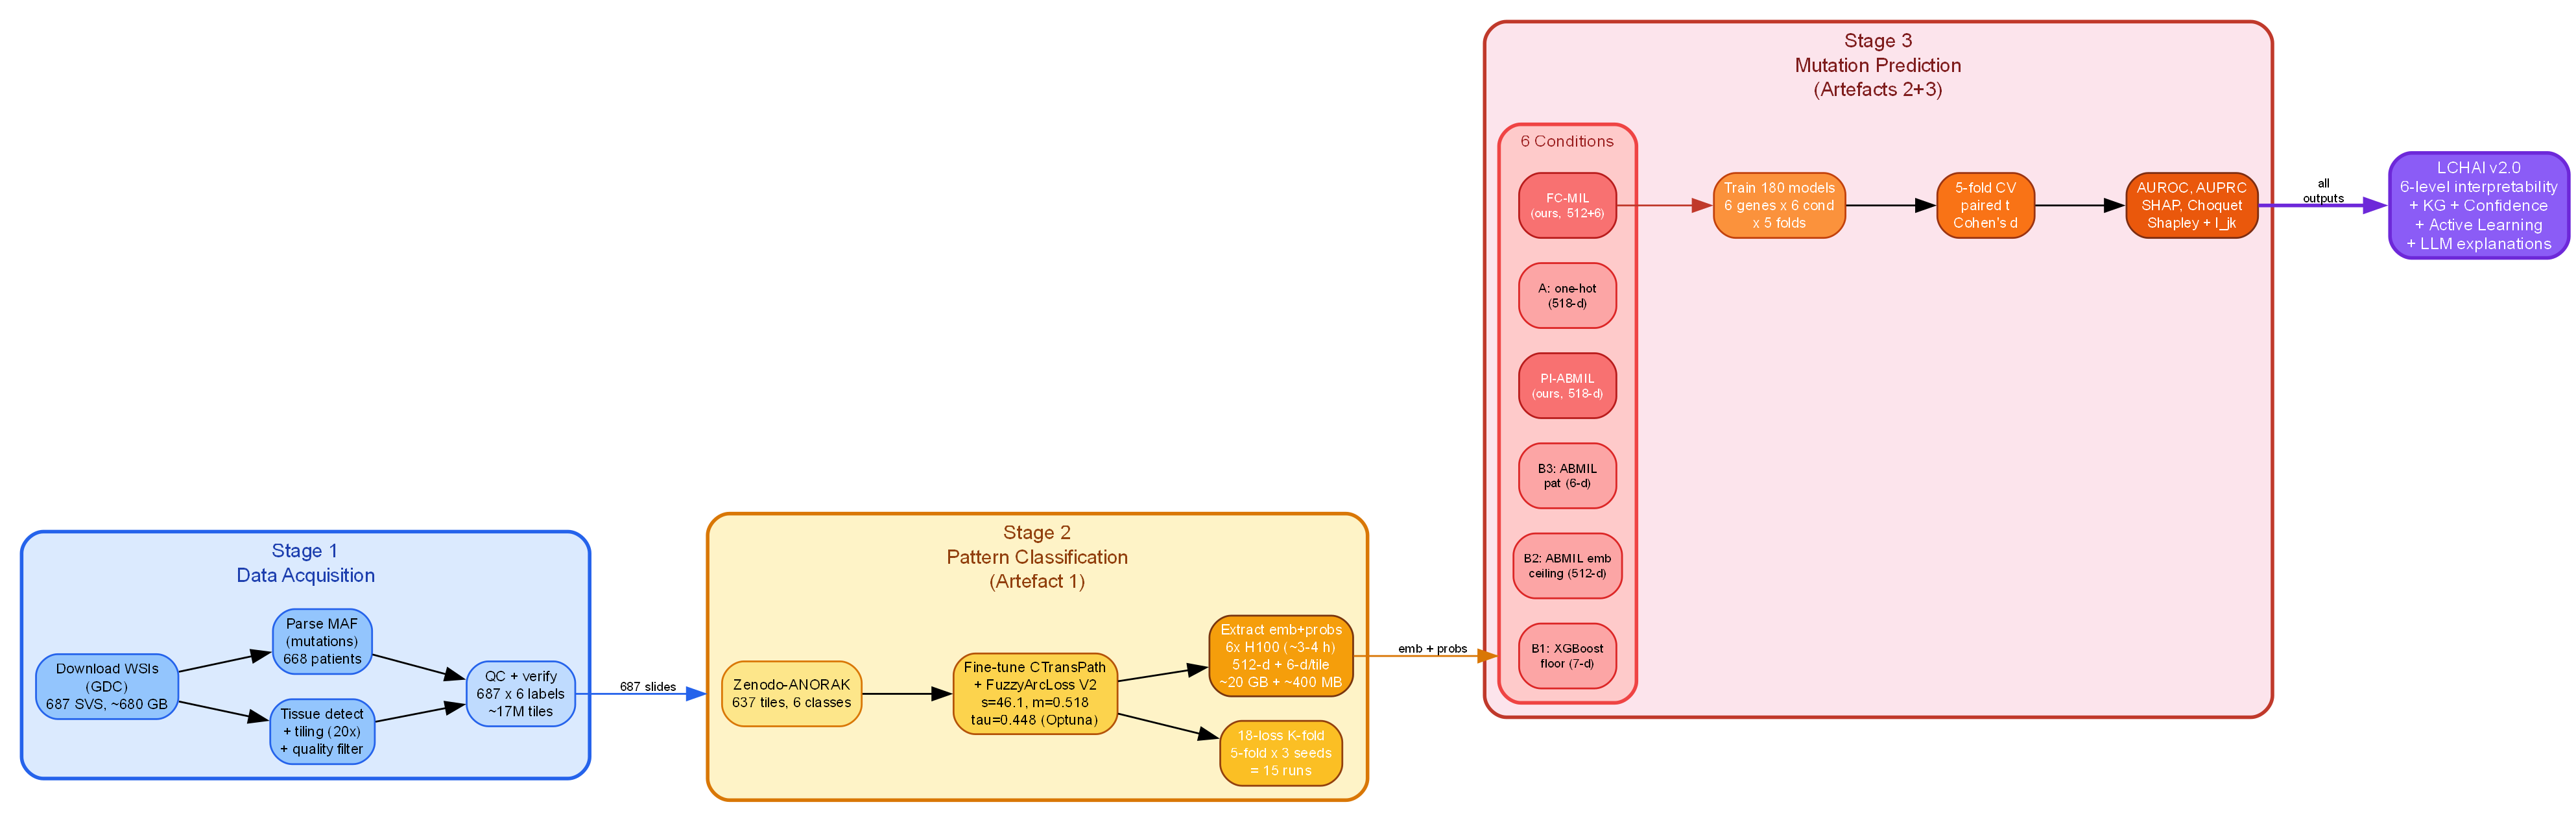
\includegraphics[width=0.92\textwidth]{chapters/figures/implementation_pipeline.png}
    \caption[Implementation pipeline]{%
        The three-stage implementation pipeline.
        \textbf{Stage~1} acquires 687 TCGA-LUAD whole-slide images
        and mutation labels from the GDC, performs tissue detection
        and tiling ($\sim$17 million tiles).
        \textbf{Stage~2} fine-tunes CTransPath with FuzzyArcLoss~V2
        on the Zenodo dataset (637 tiles, 6 classes), then extracts
        512-d embeddings and 6-d pattern probabilities for every tile
        across 6$\times$ H100 GPUs ($\sim$3--4\,h).
        \textbf{Stage~3} constructs tile-level representations for
        six experimental conditions, trains 180 models (6 genes
        $\times$ 6 conditions $\times$ 5 folds), and evaluates with
        AUROC, SHAP attributions, and Choquet Shapley values.
        The LCHAI~v2.0 prototype integrates all outputs into a
        clinical decision support interface.
        Cylinder nodes indicate persistent storage; grey annotations
        show tools and approximate computation times.}
    \label{fig:implementation_pipeline}
\end{figure}
% ============================================================================
\section{Hardware and Software Environment}
\label{sec:impl:environment}
% ============================================================================

\subsection{Computational Infrastructure}
\label{sec:impl:hardware}

All experiments were conducted on a single workstation equipped with the following hardware:

\begin{itemize}
    \item \textbf{GPU:} 6$\times$ NVIDIA H100 80\,GB HBM3 (used for embedding extraction and data-parallel multi-GPU training).
    \item \textbf{CPU:} AMD EPYC 9654 96-core processor.
    \item \textbf{RAM:} 1.5\,TB DDR5.
    \item \textbf{Storage:} 30\,TB NVMe SSD array for WSI storage and tile caching.
\end{itemize}

The H100 GPUs were used in two modes: (1)~all six GPUs simultaneously for the embedding extraction pipeline (Section~\ref{sec:impl:embedding_extraction}), which is I/O- and compute-intensive, and (2)~single-GPU training for the ABMIL and Choquet models, which are memory-light but require many sequential training runs (5 folds $\times$ 6 conditions $\times$ 6 genes = 180 training runs).

\subsection{Software Stack}
\label{sec:impl:software}

Table~\ref{tab:software_stack} lists the principal software components and their versions.

\begin{table}[ht!]
\centering
\caption{Software stack used for implementation.}
\label{tab:software_stack}
\begin{tabular}{l l l}
\hline
\textbf{Component} & \textbf{Version} & \textbf{Purpose} \\
\hline
Python & 3.10 & Primary implementation language \\
PyTorch & 2.1+ & Deep learning framework \\
torchvision & 0.16+ & Image transforms and pretrained models \\
timm & 0.9+ & CTransPath backbone (Swin Transformer) \\
OpenSlide & 4.0 & WSI reading (SVS format) \\
Kornia & 0.7+ & GPU-accelerated augmentations \\
scikit-learn & 1.3+ & StratifiedKFold, metrics \\
XGBoost & 2.0+ & Gradient-boosted tree baseline \\
Optuna & 3.4+ & Bayesian hyperparameter optimisation \\
SHAP & 0.43+ & Feature attribution \\
NumPy, Pandas & latest & Data manipulation \\
Matplotlib, Seaborn & latest & Visualisation \\
RAPIDS cuML & 23.10+ & GPU-accelerated data processing \\
\hline
\end{tabular}
\end{table}

All code was developed in Python as Jupyter notebooks (for interactive analysis) and standalone scripts (for batch execution).
Training runs were managed through shell scripts with \texttt{nohup} for long-running processes, with output logged to timestamped text files.

\subsection{Source Code Organisation}
\label{sec:impl:code_org}

The implementation is structured into four logical modules:
\begin{enumerate}
    \item \textbf{Pattern classification pipeline.}
    Fine-tuning of the CTransPath backbone with FuzzyArcLoss~V2
    on 637 expert-annotated tiles from the Zenodo--ANORAK
    dataset~\cite{anorak2024} (Section~\ref{sec:uc:zenodo}),
    including the Optuna hyperparameter search (50 trials) and the
    18-loss ablation benchmark (15 runs per loss).

    \item \textbf{Embedding extraction pipeline.}
    Batch extraction of 512-dimensional CTransPath embeddings and
    6-dimensional pattern probability vectors for all 687 slides,
    distributed across six H100 GPUs via data-parallel training.

    \item \textbf{Mutation prediction benchmark.}
    The six-condition, six-gene, five-fold cross-validation benchmark,
    including XGBoost baseline, ABMIL variants, and Fuzzy Choquet MIL.
    Ground-truth mutation labels are derived from TCGA Masked Somatic
    Mutation MAF files (Section~\ref{sec:impl:data:maf}).

    \item \textbf{LCHAI v2.0 web application.}
    A microservices architecture (Section~\ref{sec:impl:lchai})
    integrating all artefacts into a clinical decision support
    prototype with an ontology explanation layer.
\end{enumerate}

All source code, trained checkpoints, and experimental scripts are
publicly available at \url{https://github.com/slima2/lchai}~\cite{lchai_repo}.


% ============================================================================
\section{Data Acquisition and Preprocessing}
\label{sec:impl:data}
% ============================================================================

The data acquisition follows the logical order of the pipeline
(Figure~\ref{fig:implementation_pipeline}):
first, the Zenodo--ANORAK tile dataset is obtained to train the pattern
classifier (Artefact~1);
then, TCGA-LUAD whole-slide images and MAF mutation labels are downloaded
as the target dataset for mutation prediction (Artefacts~2 and~3);
finally, the TCGA slides are tiled and quality-filtered before inference.


\subsection{Zenodo--ANORAK Pattern Tile Dataset}
\label{sec:impl:data:zenodo}

The tile-level pattern classification training data were downloaded from
the Zenodo data repository (DOI: \texttt{10.5281/zenodo.10016027}),
originally published alongside the ANORAK model for LUAD growth pattern
grading~\cite{anorak2024}.
The download comprises three components
(described in detail in Section~\ref{sec:uc:zenodo}):
\begin{itemize}
    \item \textbf{H\&E image tiles} (732 PNG/JPG files at
    $224 \times 224$ pixels, $20\times$ magnification).
    \item \textbf{Pixel-level annotation masks} (731 MATLAB
    \texttt{.mat} files; one image lacks a mask), each containing an
    integer matrix where every pixel carries a growth pattern class
    label (0--6; see Table~\ref{tab:variant_types_patterns}).
    The tile-level class label is derived by majority vote over
    annotated pixels.
    The binary tissue segmentation mask used as the 4th input
    channel (Section~\ref{sec:uc:pipeline_fixes}) is extracted
    from these \texttt{.mat} files by thresholding non-zero pixels.
    \item \textbf{Colour-coded annotation overlays} (PNG files)
    used for visual verification during development but not for
    model training.
\end{itemize}

The class mapping from \texttt{.mat} integer labels to the
ANORAK pattern taxonomy follows the official Zenodo documentation
(Section~\ref{sec:uc:zenodo}).

Of the 732 raw images, 731 have annotation masks.
After excluding 94 tiles labelled as class~0 (background/other),
the final training set comprises \textbf{637 tiles across 6 ANORAK
classes} (including cribriform, label~1;
Table~\ref{tab:dataset_config_anorak}).
These 637 tiles are used exclusively to fine-tune the CTransPath
backbone with FuzzyArcLoss~V2 (Section~\ref{sec:impl:pattern});
they are \emph{not} part of the TCGA-LUAD mutation prediction dataset.


\subsection{TCGA-LUAD Slide Download}
\label{sec:impl:data:download}

Whole-slide images were downloaded from the NCI Genomic Data Commons (GDC)
using the GDC Data Transfer Tool and custom Python scripts that query the
GDC REST API.
The download pipeline performs the following steps:

\begin{enumerate}
    \item \textbf{Query the GDC API} for diagnostic whole-slide images
    from the TCGA-LUAD project.  The query restricts results to SVS-format
    files classified as diagnostic slides, excluding frozen-section and
    tissue-slide images that are unsuitable for morphological analysis.
    \item \textbf{Deduplicate} by selecting one slide per patient,
    preferring primary tumour samples (sample type code \texttt{01A})
    over recurrence or metastasis.
    Note that 19 patients in the final cohort retained more than one slide
    (e.g.\ both a diagnostic DX and a tissue-sample BS section); all such
    slides were included to maximise the usable dataset.
    \item \textbf{Download} each SVS file via the GDC data endpoint with
    retry logic (exponential backoff, maximum 5 retries).
    \item \textbf{Verify} file integrity by checking that each downloaded
    file opens successfully with OpenSlide.
\end{enumerate}

The complete TCGA-LUAD slide collection comprises \textbf{687} successfully
downloaded and verified SVS files from \textbf{668} unique patients,
totalling approximately 680\,GB of storage.

\subsection{Mutation Data Acquisition}
\label{sec:impl:data:maf}

Masked Somatic Mutation MAF files were downloaded from the GDC for the
TCGA-LUAD project (format and variant types described in
Section~\ref{sec:uc:tcga:variant_types}).
The MAF processing pipeline
extracts the following information per case:

\begin{enumerate}
    \item Parse the MAF file (tab-delimited, one variant per row).
    \item Filter to non-silent (protein-altering) variants by retaining
    only those rows whose variant classification indicates a functional
    consequence: missense mutations, nonsense mutations, frameshift
    insertions and deletions, splice-site variants, and in-frame
    insertions and deletions.  Silent (synonymous) variants are
    excluded because they do not alter the protein product.
    \item Extract the TCGA barcode from \texttt{Tumor\_Sample\_Barcode}
    (first 12 characters: \texttt{TCGA-XX-XXXX}).
    \item For each target gene $g \in \mathcal{G}$, set $Y^{(g)} = 1$ if
    at least one non-silent variant exists in that gene for the case,
    else $Y^{(g)} = 0$.
    \item Output a binary mutation label matrix: rows = cases, columns
    = genes.
\end{enumerate}

The resulting label matrix has dimensions $668 \times 6$
(all LUAD patients with available WSIs in the GDC, noting that the
GDC cohort has expanded since the initial release).
This matrix is joined to the slide inventory (687 slides from 668 patients)
to produce the final analysis dataset, with patient-level keys used to
handle the 19 patients contributing multiple slides.

\subsection{Tile Extraction}
\label{sec:impl:data:tiling}

The tiling pipeline processes each SVS file as follows:

\begin{enumerate}
    \item \textbf{Read the WSI} at $20\times$ magnification using OpenSlide.
    If the native magnification differs from $20\times$, the appropriate
    pyramid level is selected and rescaled.
    \item \textbf{Generate a tissue mask} using Otsu thresholding on a
    greyscale thumbnail, followed by H\&E hue verification and
    morphological cleanup (details in
    Section~\ref{sec:impl:data:tile_filtering}).
    \item \textbf{Extract tiles} of $224 \times 224$ pixels from
    tissue-containing regions, discarding tiles with $< 50\%$ tissue
    content.
    \item \textbf{Save tile coordinates} (not images) to avoid disk space
    explosion. Tiles are read on-the-fly during embedding extraction using
    the stored coordinates and the original SVS file.
\end{enumerate}

Across 687 slides, the pipeline identified approximately 17 million tiles
(median: $\sim$25{,}000 per slide; range: 5{,}000--80{,}000).


\subsection{Tile Quality Filtering}
\label{sec:impl:data:tile_filtering}

Not all tiles extracted from a WSI contain diagnostically relevant
tissue.
Whole-slide images routinely include background glass, pen markings
from pathologists, tissue folds, mounting medium residue, and scanner
artefacts.
If these tiles are passed to the pattern classifier or embedding
extractor, they introduce noise that degrades both pattern composition
estimates and downstream mutation predictions.
A multi-stage filtering pipeline rejects non-tissue tiles before any
model inference occurs.
Figure~\ref{fig:tile_filtering_pipeline} provides an overview of the
three-stage pipeline.

\begin{figure}[ht!]
\centering
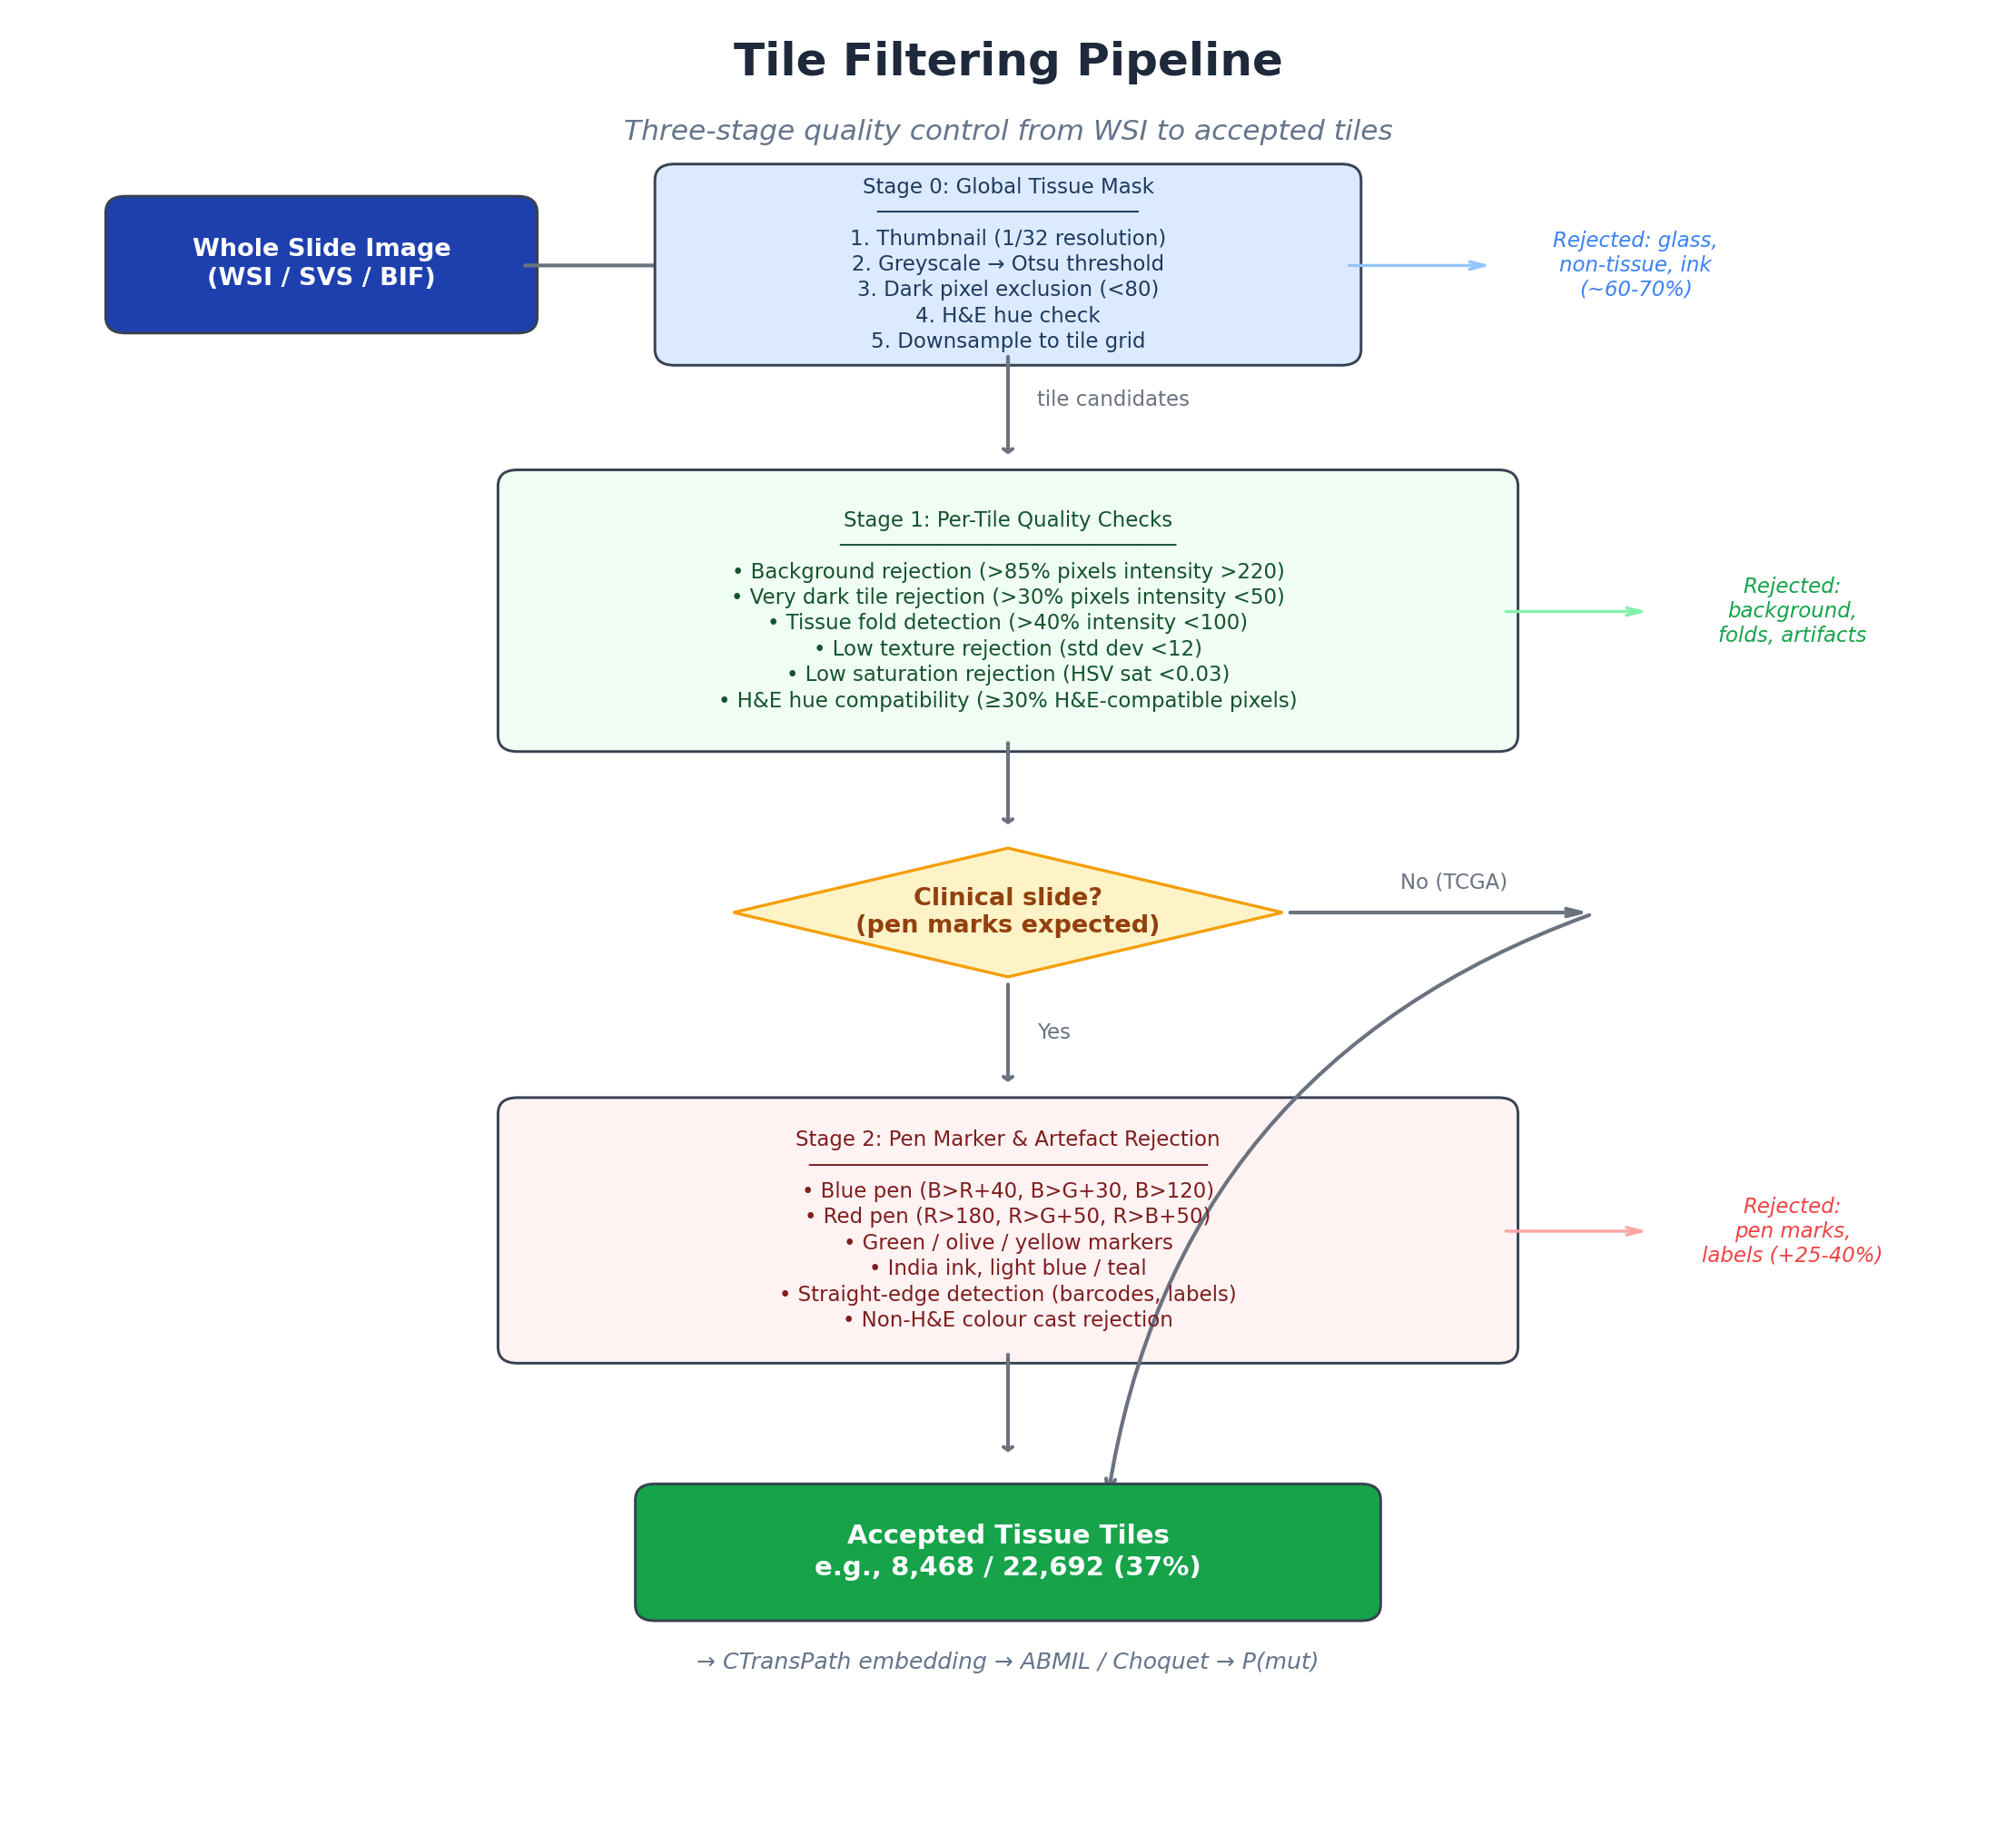
\includegraphics[width=0.92\textwidth]{chapters/figures/tile_filtering_pipeline.png}
\caption[Three-stage tile filtering pipeline]{%
    Three-stage tile filtering pipeline from WSI to accepted tissue
    tiles.
    \textbf{Stage~0} generates a global tissue mask via Otsu
    thresholding on a low-resolution thumbnail, rejecting 60--70\%
    of tile candidates (glass, non-tissue).
    \textbf{Stage~1} applies per-tile quality checks (brightness,
    texture, saturation, H\&E hue compatibility).
    \textbf{Stage~2} (clinical slides only) applies colour-specific
    filters for pen markers, labels, and non-H\&E artefacts.
    On the representative case TCGA-49-AAR9, 8{,}468 of 22{,}692
    tile candidates (37\%) pass all filters.}
\label{fig:tile_filtering_pipeline}
\end{figure}

\subsubsection{Stage 0: Global Tissue Mask (Otsu Thresholding)}

Before individual tiles are read, a binary tissue mask is computed on a
low-resolution thumbnail (1/32 of the full WSI dimensions):

\begin{enumerate}
    \item The thumbnail is converted to greyscale by averaging the RGB
    channels.
    \item Otsu's method~\cite{otsu1979threshold}---an automatic
    thresholding algorithm that selects the intensity value maximising
    the between-class variance of the resulting two pixel
    groups---determines an optimal intensity threshold $t^{*}$ that
    separates tissue (dark/coloured) from glass (white).
    \item Pixels with intensity $< t^{*}$ are tentatively marked as
    tissue.
    \item Two refinements are applied:
    \begin{itemize}
        \item Very dark pixels (intensity $< 80$) are excluded---these
        typically correspond to ink marks on glass rather than stained
        tissue.
        \item An H\&E hue check retains only pixels whose colour is
        consistent with eosin (pink, $R > G$) or haematoxylin (purple,
        $R \approx B > G$), rejecting non-H\&E colours such as blue
        pen ink or green marker.
    \end{itemize}
    \item The resulting mask is downsampled to tile-grid resolution.
    Tile candidates that fall outside the mask are skipped without
    reading from the WSI file, which significantly reduces I/O.
\end{enumerate}

\subsubsection{Stage 1: Per-Tile Brightness, Texture and Colour Checks}

Each tile that passes the global mask is subjected to pixel-level
quality checks:

\begin{description}
    \item[Background rejection.]
    Tiles where fewer than 15\% of pixels have greyscale intensity
    $< 220$ are discarded as predominantly white background.

    \item[Very dark tile rejection.]
    Tiles where $> 30\%$ of pixels have intensity $< 50$ are
    discarded---these correspond to scanning artefacts, out-of-focus
    regions, or residual ink.

    \item[Tissue fold detection.]
    Tissue folds produce unnaturally dark, double-stained regions.
    Tiles are rejected if $> 40\%$ of pixels have intensity $< 100$,
    or if the mean greyscale is below 120 with $> 25\%$ of pixels
    below 100.

    \item[Low texture rejection.]
    Real tissue exhibits high intensity variance due to the mix of
    nuclei, stroma, and glandular lumina.
    Tiles with greyscale standard deviation $< 12$ are rejected as
    featureless (empty lumina, glass, mounting medium).

    \item[Low saturation rejection.]
    Tiles with mean saturation $< 0.03$ in the HSV colour space
    (Hue--Saturation--Value, which separates chromatic content from
    brightness) lack meaningful staining and are rejected.

    \item[H\&E hue compatibility.]
    A per-tile hue filter verifies that at least 30\% of pixels are
    compatible with H\&E staining: pink ($R > G$, $R > B - 30$,
    saturation $> 0.03$), purple ($B > G$, $R > G - 15$,
    saturation $> 0.03$), or pale tissue (greyscale $> 180$,
    saturation $< 0.15$).
    This filter catches pen-ink tiles and non-H\&E special stains
    that pass brightness checks because they are neither white nor
    dark, while tolerating lightly stained tissue.
\end{description}

For the TCGA benchmark, Stages~0 and~1 are sufficient because the
curated slides contain no pen markings.
An additional Stage~2 (pen marker and artefact rejection) is applied
in the LCHAI~v2.0 clinical deployment to handle hospital slides with
pathologist annotations; it is described in
Section~\ref{sec:impl:lchai:pen_filters}.

\paragraph{Impact on downstream performance.}
The filtering pipeline typically rejects 15--25\% of tile candidates
on curated TCGA slides.
By removing non-tissue tiles, the pattern composition estimates
become more accurate (no background tiles classified as a histological
pattern), and the attention mechanism in Artefacts~2 and~3 operates on
a cleaner bag of instances, reducing noise in mutation predictions.


% ============================================================================
\section{Implementation of Artefact 1: FuzzyArcLoss V2 Pattern Classifier}
\label{sec:impl:pattern}
% ============================================================================

\subsection{Network Architecture}
\label{sec:impl:pattern:arch}

The pattern classifier consists of three components:

\begin{enumerate}
    \item \textbf{Backbone:} CTransPath (Swin Transformer + CNN stem), loaded from the pretrained checkpoint. The first convolutional layer is expanded from 3 to 4 input channels (Section~\ref{sec:meth:mask_channel}) by duplicating and averaging the pretrained weights for the mask channel.

    \item \textbf{Projection head:} A single linear layer $\mathbb{R}^{768} \to \mathbb{R}^{512}$ followed by batch normalisation and $\ell_2$ normalisation. The output lies on the unit hypersphere $\mathbb{S}^{511}$.

    \item \textbf{Angular margin classifier:} The \texttt{FuzzyArcLossV2} module maintains a $6 \times 512$ weight matrix $\mathbf{W}$ (one prototype per class). During the forward pass, the module:
    \begin{enumerate}
        \item $\ell_2$-normalises both $\mathbf{W}$ and the input embedding.
        \item Computes $\cos\theta_k = \tilde{\mathbf{w}}_k^\top \tilde{\mathbf{x}}$ for all $k$.
        \item Computes the fuzzy membership $\mu_i$ according to Equation~\ref{eq:membership_v2}.
        \item Computes the ArcFace target logit $\phi_i = \cos(\theta_y + m)$ and interpolates: $\tilde{z}_{y,i} = \mu_i \, \phi_i + (1 - \mu_i) \, \cos\theta_y$ (Equation~\ref{eq:fuzzyarcloss_v2_method}).
        \item Scales all logits by $s$ and returns both the interpolated logits (for training) and the margin-free logits (for evaluation).
    \end{enumerate}
\end{enumerate}

The total parameter count is approximately 28 million (dominated by the CTransPath backbone), of which 3{,}072 are prototype parameters and 393{,}728 are projection head parameters.

\subsection{FuzzyArcLoss V2 Module: Implementation Details}
\label{sec:impl:pattern:fuzzy_module}

The core of the FuzzyArcLoss~V2 implementation handles the numerical challenges specific to angular margin computation in fp32 arithmetic:

\begin{enumerate}
    \item \textbf{Numerical clipping:} The cosine similarity is clipped to $[-1 + \epsilon, 1 - \epsilon]$ with $\epsilon = 10^{-7}$ before applying $\arccos$ to prevent NaN gradients at the boundaries.

    \item \textbf{ArcFace logit with boundary correction:} The target angle $\hat{\theta}_y = \theta_y + m$ may exceed $\pi$, producing $\cos\hat{\theta}_y < -1$. A boundary correction is applied: if $\cos\theta_y < \cos(\pi - m)$, the ArcFace logit $\phi_i$ is computed in the cosine domain ($\cos\theta_y - m \sin m$) as a numerically stable fallback. The interpolation $\tilde{z}_{y,i} = \mu_i \phi_i + (1-\mu_i) \cos\theta_y$ is applied after this correction.

    \item \textbf{One-hot masking:} The interpolated logit replaces only the correct-class entry via one-hot masking of the logit matrix, ensuring that negative classes retain their unmodified $s \cos\theta_k$ logits.
\end{enumerate}

\subsection{Loss Function Variants Implemented}
\label{sec:impl:pattern:losses}

In total, 18 loss function variants were implemented for the ablation study.
Table~\ref{tab:loss_variants} lists the complete set.

\begin{table}[ht!]
\centering
\small
\caption{All 18 loss function variants implemented for the pattern classification ablation. Default hyperparameters are listed where applicable.}
\label{tab:loss_variants}
\begin{tabular}{r l l}
\hline
\textbf{\#} & \textbf{Loss function} & \textbf{Key parameters} \\
\hline
1  & Softmax Cross-Entropy & --- \\
2  & Label Smoothing CE & $\epsilon = 0.1$ \\
3  & Focal Loss & $\gamma = 2$, $\alpha = $ class-balanced \\
4  & ArcFace & $s = 30$, $m = 0.5$ \\
5  & CosFace & $s = 30$, $m = 0.35$ \\
6  & SphereFace & $s = 30$, $m = 4$ (integer) \\
7  & AdaptiveFace & $s = 30$, $m = 0.5$ \\
8  & Combined Margin (Arc+Cos) & $s = 30$, $m_1 = 0.3$, $m_2 = 0.2$ \\
9  & FuzzyArcLoss V1 & $s = 30$, $m = 0.5$, linear $\mu$ \\
10 & FuzzyArcLoss V2 (default) & $s = 30$, $m = 0.5$, $\tau = 0.5$ \\
11 & FuzzyArcLoss V2 (Optuna) & $s = 46.1$, $m = 0.518$, $\tau = 0.448$ \\
12 & FuzzyArcLoss V2 ClassParams & Per-class $m_k$, $\tau_k$ \\
13 & FuzzyArcLoss V3 SubCenters & $C = 4$, $s = 30$, $m = 0.5$ \\
14 & FuzzyArcLoss V3 (Optuna) & $C = 4$, Optuna-tuned \\
15 & FuzzyCosFace V2 & Cosine margin with fuzzy $\mu$ \\
16 & FuzzySphereFace V2 & Multiplicative margin with fuzzy $\mu$ \\
17 & Triplet + Angular & Combined metric learning \\
18 & Center Loss + Softmax & Center loss $\lambda = 0.003$ \\
\hline
\end{tabular}
\end{table}

All 18 variants share the same backbone architecture, projection head, training protocol, and augmentation pipeline, differing only in the loss computation module.
This design ensures that performance differences are attributable to the loss function alone.

\subsection{Embedding Extraction Pipeline}
\label{sec:impl:embedding_extraction}

After training the pattern classifier, the CTransPath backbone and
projection head are frozen and used to extract embeddings and pattern
predictions for every tile of every TCGA-LUAD slide.
The extraction pipeline is the most
compute-intensive stage:

\begin{enumerate}
    \item \textbf{Load the trained model} from the best FuzzyArcLoss~V2
    checkpoint and set it to evaluation mode. The angular margin module is bypassed;
    only the backbone and projection head are used.

    \item \textbf{Distribute across GPUs} using data-parallel replication
    over the 6 available H100 GPUs. Each GPU processes a batch of tiles
    independently.

    \item \textbf{For each slide}, read tiles on-the-fly from the SVS file
    using the stored coordinates and OpenSlide. Tiles are batched
    (batch size = 256 per GPU, effective batch size = 1{,}536 across 6 GPUs),
    normalised with ImageNet statistics, and passed through the model.

    \item \textbf{Store two outputs per tile:}
    \begin{itemize}
        \item The 512-dimensional embedding $\mathbf{x}_i$ (after projection
        head, before $\ell_2$ normalisation).
        \item The 6-dimensional pattern probability vector $\mathbf{p}_i$
        (softmax of the margin-free logits).
    \end{itemize}

    \item \textbf{Save per-slide arrays}: embedding vectors
    ($N_s \times 512$, float16 for storage efficiency) and
    pattern probability vectors ($N_s \times 6$, float32).
\end{enumerate}

\textbf{Computational cost.}
Extracting embeddings for all 687 LUAD slides ($\sim$17 million tiles) % <-- CHANGED: 505→687, 12.6M→17M
required approximately 3--4 hours on 6$\times$ H100 GPUs. % <-- CHANGED: 2–3→3–4 h (more tiles)
The resulting data occupies approximately 20\,GB (embeddings in float16) % <-- CHANGED: 15→~20 GB
plus 400\,MB (pattern probabilities in float32). % <-- CHANGED: 300→~400 MB


\subsection{Data Completeness Verification}
\label{sec:impl:data_completeness}

An automated verification step confirmed that all 687 LUAD slides have
both embedding and pattern probability files and appear in the mutation
label matrix, ensuring 100\% data completeness for the downstream
benchmark.

% ============================================================================
\section{Implementation of Artefact 2: Pattern-Informed ABMIL}
\label{sec:impl:mutation}
% ============================================================================

\subsection{Benchmark Input Preparation}
\label{sec:impl:mutation:prep}

The benchmark input preparation module performs
the following steps:

\begin{enumerate}
    \item \textbf{Parse MAF files} for LUAD and LUSC, extracting the binary
    mutation matrix for the six target genes.
    \item \textbf{Classify slides} by cancer type using the TCGA barcode
    (cross-referencing with the LUAD and LUSC MAFs).
    \item \textbf{Filter to LUAD-only:} 687 slides matched to the LUAD MAF; % <-- CHANGED: 505→687
    LUSC slides were excluded at this stage
    (the mixed-cohort experiment with 150 LUSC slides was an earlier
    exploratory analysis documented in Section~\ref{sec:uc:tcga:luad_only}). % <-- CHANGED: clarified
    \item \textbf{Build a slide-level data structure}
    containing, for each slide: the case ID, the patient ID (first 12
    characters of the TCGA barcode), the path to the embeddings file, % <-- NEW: patient ID added
    the path to the pattern probabilities file, and the mutation labels
    for all six genes.
\end{enumerate}

\subsection{ABMIL Network Implementation}
\label{sec:impl:mutation:network}

The ABMIL model has a configurable input dimension to accommodate the different experimental conditions.
The architecture follows the specification in Section~\ref{sec:meth:mutation:abmil}:

The ABMIL module implements four stages: (i)~a linear encoder that
projects the input from its condition-specific dimension to 256
hidden units with layer normalisation, ReLU activation, and dropout;
(ii)~a gated attention mechanism that computes per-tile importance
weights; (iii)~attention-weighted aggregation into a single
slide-level vector; and (iv)~a linear classifier that produces one
mutation logit per gene.

The input dimension varies by condition: 512 (B2), 6 (B3), 518 (PI-ABMIL and A).
A separate model instance is created and trained for each (condition, gene) pair.

\subsection{Training Configuration}
\label{sec:impl:mutation:training}

Each ABMIL model is trained with the following configuration:

\begin{itemize}
    \item \textbf{Optimiser:} Adam with learning rate $2 \times 10^{-4}$ and weight decay $10^{-5}$.
    \item \textbf{Learning rate schedule:} Cosine annealing with warm restarts (restart period $T_0 = 10$ epochs).
    \item \textbf{Epochs:} 50 with early stopping (patience = 15 epochs, monitored on validation AUROC).
    \item \textbf{Batch size:} 1 slide per batch (standard in MIL, as each slide has a variable number of tiles).
    \item \textbf{Loss:} Binary cross-entropy with logits (applied to raw model outputs before sigmoid).
    \item \textbf{Gradient accumulation:} 4 slides before each optimiser step, to stabilise gradients given the batch size of 1.
\end{itemize}

\textbf{Tile sampling.}
For slides with more than 4{,}096 tiles, a random subsample of 4{,}096 tiles is drawn at each training epoch to limit memory consumption and introduce stochastic regularisation.
At evaluation, all tiles are used.

Table~\ref{tab:hyper_abmil2} summarises the complete hyperparameter
configuration for the ABMIL mutation prediction benchmark.
 
\begin{table}[ht!]
\centering
\small
\caption{Hyperparameters for the ABMIL mutation prediction benchmark
(conditions B2, B3, PI-ABMIL~(ours), A).}
\label{tab:hyper_abmil2}
\begin{tabular}{l l c}
\hline
\textbf{Parameter} & \textbf{Description} & \textbf{Value} \\
\hline
Embedding dim.      & CTransPath projection output        & 512 \\
Pattern dim.        & FuzzyArcLoss~V2 soft probabilities  & 6 \\
Concat dim.         & Total input (PI-ABMIL condition PI, ours)  & 518 \\
Attention hidden    & Gated attention hidden size         & 256 \\
Attention dim       & $\mathbf{w}$, $\mathbf{V}$, $\mathbf{U}$ size & 128 \\
Dropout             & After attention and encoder         & 0.25 \\
Learning rate       &                                     & 2e-4 \\
Weight decay        &                                     & 1e-5 \\
Epochs              & Maximum training epochs             & 50 \\
Early stopping      & Patience (validation AUROC)         & 15 \\
Optimiser           &                                     & Adam \\
LR scheduler        & Cosine annealing (warm restarts) $T_0$   & 10 epochs \\
Loss function       & Binary cross-entropy with logits    & Sigmoid + CE \\
Batch size          & Slides per batch                    & 1 \\
Gradient accumulation & Steps before optimiser update    & 4 \\
Max tiles per slide & Subsampled during training          & 4{,}096 \\
Folds               & Patient-stratified $K$-fold         & 5 \\
Seed                &                                     & 42 \\
\hline
\end{tabular}
\end{table}


\subsection{Benchmark Execution}
\label{sec:impl:mutation:benchmark}

The benchmark runner orchestrates the complete evaluation:

\begin{enumerate}
    \item \textbf{Outer loop:} For each gene $g \in \mathcal{G}$
    (6 genes).
    \item \textbf{Middle loop:} For each experimental condition
    $c \in \{B1, B2, B3, \text{PI-ABMIL}, A, \text{FC-MIL}\}$ (6 conditions).
    \item \textbf{Inner loop:} For each fold $k \in \{1, \ldots, 5\}$
    (5-fold patient-stratified CV). % <-- CHANGED: added "patient-stratified"
    \begin{enumerate}
        \item Split the 668 patients into train ($\sim$534) and test
        ($\sim$134), using stratified $K$-fold splitting on % <-- CHANGED: 505→668 patients, 404→534, 101→134
        the binary mutation label for gene $g$.
        All slides from a given patient are assigned to the same
        fold to prevent data leakage. % <-- NEW: explains patient-level constraint
        This yields approximately 549 training slides and 138 test
        slides per fold (exact counts vary by fold due to the
        19 multi-slide patients). % <-- NEW: slide counts clarified
        \item Construct the tile-level representations $\mathbf{h}_i$
        according to the condition
        (Table~\ref{tab:tile_representations}).
        \item For condition B1: train an XGBoost classifier on the
        7 slide-level features.
        \item For conditions B2, B3, PI-ABMIL, A: train an ABMIL model for
        50 epochs.
        \item For condition FC-MIL: train the Fuzzy Choquet MIL model for
        50 epochs.
        \item Evaluate on the test fold: compute AUROC, AUPRC,
        and F1 at threshold 0.5.
        \item Save per-fold predictions and metrics as JSON.
    \end{enumerate}
    \item \textbf{Aggregate:} Compute mean $\pm$ std across 5 folds
    for each (gene, condition) pair.
    \item \textbf{Statistical tests:} Paired $t$-tests and Cohen's $d$
    between all condition pairs.
\end{enumerate}

\textbf{Computational cost.}
The complete benchmark (6 genes $\times$ 6 conditions $\times$ 5 folds
= 180 model trainings) required approximately 15--16 hours on 6
H100 GPUs running in parallel (one gene per GPU).
Wall-clock time was dominated by RBM10, whose low prevalence (37
positive slides, 5.4\%) caused the ABMIL models to train for the full
50 epochs before early stopping, at approximately 30 minutes per
(condition, fold) pair for that gene.
The Fuzzy Choquet condition trains in $\sim$3 minutes per fold
compared to $\sim$8 minutes for the standard ABMIL conditions,
despite comparable parameter counts, because the Choquet integral
computation over 6 pattern dimensions is cheaper than the
full-dimensional attention over 518-d concatenated representations.



\subsection{XGBoost Baseline Implementation}
\label{sec:impl:mutation:xgboost}

The XGBoost baseline (condition B1) operates on slide-level features rather than tile-level representations.
For each slide, the seven features (six pattern fractions + entropy) are computed from the pre-extracted pattern probabilities:

\begin{verbatim}
for slide in slides:
    probs = np.load(slide.pattern_probs_path)   # (N_tiles, 6)
    labels = probs.argmax(axis=1)                # (N_tiles,)
    fracs = np.bincount(labels, minlength=6) / len(labels)
    entropy = -np.sum(fracs * np.log(fracs + 1e-8))
    features[slide.id] = np.append(fracs, entropy)
\end{verbatim}

The XGBoost classifier is trained with the hyperparameters listed in Table~\ref{tab:hyper_xgboost2} (\texttt{max\_depth=4}, \texttt{n\_estimators=300}, \texttt{learning\_rate=0.05}, \texttt{scale\_pos\_weight} set to the class imbalance ratio).
TreeSHAP is applied post-training to compute per-feature attributions.

Table~\ref{tab:hyper_xgboost2} summarises the XGBoost baseline
hyperparameters.
 
\begin{table}[ht!]
\centering
\small
\caption{Hyperparameters for the XGBoost baseline (condition~B1).}
\label{tab:hyper_xgboost2}
\begin{tabular}{l l c}
\hline
\textbf{Parameter} & \textbf{Description} & \textbf{Value} \\
\hline
Input features      & 6 pattern percentages + entropy     & 7 \\
\texttt{n\_estimators}  &                                 & 300 \\
\texttt{max\_depth}     &                                 & 4 \\
\texttt{learning\_rate} &                                 & 0.05 \\
\texttt{scale\_pos\_weight} & Class imbalance correction  & auto \\
\texttt{eval\_metric}   &                                 & logloss \\
Early stopping      & Rounds without improvement          & 30 \\
Random state        &                                     & 42 \\
\hline
\end{tabular}
\end{table}
 

% ============================================================================
\section{Implementation of Artefact 3: Fuzzy Choquet MIL}
\label{sec:impl:choquet}
% ============================================================================

\subsection{Choquet Integral Module}
\label{sec:impl:choquet:module}

The Choquet integral is implemented as a differentiable PyTorch module to enable end-to-end training with backpropagation.
The key implementation challenge is that the Choquet integral requires sorting the input vector and evaluating the fuzzy measure on nested subsets, which involves discrete operations.

The implementation follows a three-step procedure for each input vector $\mathbf{x} \in \mathbb{R}^6$:

\begin{enumerate}
    \item \textbf{Sort:} Obtain the permutation $\sigma$ such that $x_{\sigma(1)} \leq x_{\sigma(2)} \leq \ldots \leq x_{\sigma(6)}$. Implemented using \texttt{torch.sort}, which provides gradients through the sorted values.

    \item \textbf{Evaluate the fuzzy measure:} For each $i = 1, \ldots, 6$, compute $g(A_i)$ where $A_i = \{\sigma(i), \sigma(i+1), \ldots, \sigma(6)\}$ is the set of indices with values $\geq x_{\sigma(i)}$. Using the 2-additive parameterisation:
    \begin{equation*}
        g(A_i) = \sum_{k \in A_i} \phi_k + \sum_{\{j,k\} \subseteq A_i} I_{jk}.
    \end{equation*}
    This is computed as a sum over the Shapley values and interaction indices for the elements in $A_i$.

    \item \textbf{Integrate:} Compute the Choquet integral as:
    \begin{equation*}
        \mathcal{C}_g(\mathbf{x}) = \sum_{i=1}^{6} (x_{\sigma(i)} - x_{\sigma(i-1)}) \cdot g(A_i),
    \end{equation*}
    with $x_{\sigma(0)} = 0$.
\end{enumerate}

All operations are differentiable, and gradients flow back through the Shapley values $\psi_k$ (unconstrained parameters before softmax) and the interaction indices $I_{jk}$.

\subsection{Fuzzy Measure Parameterisation}
\label{sec:impl:choquet:measure}

The Shapley values are parameterised via softmax to ensure non-negativity and normalisation:

The fuzzy measure stores 6 singleton importance values (Shapley
parameters) and 15 pairwise interaction weights as unconstrained
learnable parameters.
At inference time, the Shapley values are normalised via softmax,
and the interaction indices are regularised toward zero during
training (Equation~\ref{eq:interaction_reg}).

\subsection{Monotonicity Constraint}
\label{sec:impl:choquet:monotonicity}

A fuzzy measure must satisfy monotonicity: $A \subseteq B \implies g(A) \leq g(B)$.
With a 2-additive parameterisation, this is not automatically guaranteed.
A soft monotonicity penalty is added to the loss function:
\begin{equation}
\label{eq:mono_penalty}
\mathcal{R}_{\text{mono}} = \lambda_M \sum_{A \subset B} \max(0, g(A) - g(B)),
\end{equation}
with $\lambda_M = 0.1$.
Enumerating all subset pairs for $n = 6$ is feasible ($2^6 = 64$ subsets), though in practice only a random sample of 100 subset pairs is evaluated per batch to reduce computational cost.

Table~\ref{tab:hyper_choquet2} summarises the Fuzzy Choquet MIL
hyperparameters.
 
\begin{table}[ht!]
\centering
\small
\caption{Hyperparameters for the Fuzzy Choquet MIL (FC-MIL, ours; condition~FC).
The \emph{interpretable} fuzzy measure has 21 learnable parameters;
the full dual-pathway model has $\sim$266{,}000.}
\label{tab:hyper_choquet2}
\begin{tabular}{l l c}
\hline
\textbf{Parameter} & \textbf{Description} & \textbf{Value} \\
\hline
\multicolumn{3}{l}{\textit{Fuzzy measure (interpretable component --- 21 params)}} \\
Number of criteria  & Histological patterns (input dim)   & 6 \\
Interaction order   & 2-additive approximation            & 2 \\
Shapley parameters  & Learnable per-pattern importance    & 6 \\
Interaction params  & Learnable pairwise interactions     & 15 \\
Interaction reg.    & L1 on interaction terms $\lambda_I$ & 0.01 \\
Monotonicity reg.   & Soft penalty weight $\lambda_M$     & 0.1 \\
Choquet scale       & Learnable scale parameter           & 10.0 (init) \\
\hline
\multicolumn{3}{l}{\textit{Embedding pathway (shared with ABMIL)}} \\
Encoder             & Linear($512 \to 256$) + LayerNorm   & 131{,}840 params \\
Gated attention     & $\mathbf{V}$, $\mathbf{U}$: $256 \to 128$; $\mathbf{w}$: $128 \to 1$ & 65{,}920 params \\
\hline
\multicolumn{3}{l}{\textit{Merge and classifier}} \\
Projection          & Linear($262 \to 256$) + LayerNorm   & 67{,}840 params \\
Classifier          & Linear($256 \to 1$)                 & 257 params \\
\hline
\multicolumn{3}{l}{\textit{Training configuration}} \\
Dropout             &                                     & 0.25 \\
Learning rate       &                                     & 2e-4 \\
Epochs              & Maximum training epochs             & 50 \\
Early stopping      & Patience (validation AUROC)         & 15 \\
Optimiser           &                                     & AdamW \\
\hline
\textbf{Total params} & \textbf{Full model}              & \textbf{$\sim$266{,}k} \\
\hline
\end{tabular}
\end{table}

% ============================================================================
\section{Integrative System: LCHAI v2.0}
\label{sec:impl:lchai}
% ============================================================================

LCHAI (Lung Cancer Histopathology AI) is an integrative clinical decision support prototype that demonstrates the translational potential of the three artifacts.
Version~1.2, implemented as a web-based application, integrates the following components.

\subsection{System Architecture}
\label{sec:impl:lchai:arch}

LCHAI follows a modular architecture with four processing layers:

\begin{enumerate}
    \item \textbf{Slide processing layer:} Accepts an uploaded SVS file, performs tiling, and extracts CTransPath embeddings and pattern probabilities using the frozen Artifact~1 model.

    \item \textbf{Analysis layer:} Runs the Pattern-Informed ABMIL (Artifact~2) and optionally the Fuzzy Choquet MIL (Artifact~3) to produce mutation predictions for all six target genes. Additionally computes slide-level pattern distribution statistics.

    \item \textbf{Interpretability layer:} Generates attention heatmaps (Level~1), pattern overlay maps (Level~2), SHAP decompositions (Level~3), Choquet Shapley values (Level~4, for FC-MIL genes), and per-slide feature channel ablation comparisons (Level~5, Section~\ref{sec:meth:interp:ablation}) that run the B2 and B3 checkpoints alongside the primary model on the same tile set to measure whether adding pattern features helps or harms the prediction on each individual slide.

    \item \textbf{Knowledge layer:} Links mutation predictions to a biomedical knowledge graph encoding gene $\to$ pathway $\to$ drug associations, and provides literature references through a DeepSearch module that queries PubMed and bioRxiv.
\end{enumerate}

\subsection{Clinical Slide Filtering: Pen Marker and Artefact Rejection}
\label{sec:impl:lchai:pen_filters}

Clinical slides frequently carry pathologist annotations (pen marks,
circled regions, case identifiers) that are absent from curated
research cohorts such as TCGA.
When processing hospital slides, LCHAI applies an additional
colour-specific filtering stage (Stage~2) beyond the universal
tissue mask and brightness checks described in
Section~\ref{sec:impl:data:tile_filtering}:

\begin{description}
    \item[Blue pen.]
    $(B > R + 40) \wedge (B > G + 30) \wedge (B > 120)$; rejected if
    $> 10\%$ of pixels match.

    \item[Red pen.]
    $(R > 180) \wedge (R > G + 50) \wedge (R > B + 50)$; rejected if
    $> 15\%$ of pixels match.

    \item[Green marker.]
    $(G > R + 30) \wedge (G > B + 30)$; rejected if $> 25\%$ of
    pixels match.

    \item[Olive/yellow marker.]
    $(R > 160) \wedge (G > 140) \wedge (B < 80) \wedge
    (R + G > 3.0B)$; rejected if $> 20\%$.

    \item[Light blue / pale blue / teal.]
    Separate filters for these hues, with thresholds between 20\% and
    50\% depending on colour specificity.

    \item[India ink.]
    Dark marks with slight blue cast (intensity $< 60$, $B > 0.8R$);
    rejected if $> 12\%$.

    \item[Straight-edge detection.]
    High directional gradient asymmetry (ratio $> 3.0$) detects
    barcodes, printed labels, and coverslip edges.

    \item[Non-H\&E colour cast.]
    Tiles where fewer than 30\% of pixels have a red component
    exceeding the blue component by at least 30 are rejected as
    incompatible with H\&E staining.
\end{description}

The thresholds were calibrated empirically on a set of 12 hospital
slides containing diverse pen colours and artefacts, with the
requirement that $< 1\%$ of true tissue tiles are falsely rejected.
On clinical slides, this stage rejects an additional 25--40\% of
tile candidates beyond Stages~0 and~1.

Additionally, the pattern overlay is clipped to a per-pixel tissue
mask derived from the original image (pixels with greyscale
intensity $< 220$), preventing the Gaussian-smoothed colour overlay
from bleeding onto white background regions.


\subsection{Confidence Calibration}
\label{sec:impl:lchai:confidence}

LCHAI labels each mutation prediction as ``Conclusive'' or ``Inconclusive'' based on the per-class reliability estimated from the K-fold evaluation.
The threshold is set at AUROC~$= 0.70$, following the widely adopted
Hosmer--Lemeshow classification~\cite{hosmer2000applied} which defines
AUROC in the range $[0.70, 0.80)$ as \emph{acceptable discrimination}
(Table~5.2 in the original reference).
Below 0.70, the model's ranking ability is considered insufficient
for clinical decision support, even as a screening tool.

\begin{itemize}
    \item \textbf{Conclusive} ($\geq 0.70$ AUROC in K-fold): TP53, EGFR. The prediction is presented with the confidence score.
    \item \textbf{Inconclusive} ($< 0.70$ AUROC in K-fold): KRAS, STK11, KEAP1, RBM10. The prediction is presented with a disclaimer: ``This gene's mutation status cannot be reliably predicted from histological features alone. Molecular testing is recommended.''
\end{itemize}

The cribriform pattern class is further flagged with a ``moderate confidence'' indicator (per-class F1 = 83.6\% in K-fold), alerting the pathologist that cribriform-dominant regions have higher classification uncertainty.

\subsection{User Interface}
\label{sec:impl:lchai:ui}

LCHAI~v2.0 presents a tabbed web interface deployed at
\texttt{https://lchai.gptfy.biz}, accessible via Keycloak-authenticated
login.  Role-based access control is managed by Keycloak (realm
\texttt{oncology}), supporting \texttt{clinician}, \texttt{admin},
and \texttt{auditor} roles.
The interface consists of four principal tabs---\emph{Analysis},
\emph{Viewer}, \emph{Graph}, and
\emph{Admin}---each described below with reference to case
TCGA-99-8025-01A-01-TS1.

\subsubsection{Analysis Tab}
\label{sec:impl:lchai:ui:analysis}

The Analysis tab (Figure~\ref{fig:lchai_v2_images}) is the primary
clinical dashboard, integrating image upload, mutation prediction results,
and multi-level explainability into a single unified view.
It is organised into gene sub-tabs sorted by descending $P(\text{mut})$,
with the highest-probability mutation selected by default.
Each gene sub-tab presents the following components:

\textbf{Component~1 --- Gene Header.}
Displays the gene name, $P(\text{mut})$ as a percentage, a confidence label (\emph{Conclusive} if fold-AUROC~$\geq 0.70$, \emph{Inconclusive} otherwise), the prediction method (B2 embeddings, PI-ABMIL, or FC-MIL), and the model AUROC.

\textbf{Component~2 --- Side-by-Side Visual Overlays.}
Two images are displayed simultaneously: (i)~a \emph{Pattern Overlay} showing the tile-level categorical colour map of the six growth patterns with a legend listing each pattern name and its composition percentage; and (ii)~an \emph{ABMIL Attention Heatmap} showing the spatial distribution of gated attention weights (top-200 tiles highlighted).
Both images support interactive hover: hovering over the pattern overlay displays the tile's classified pattern; hovering over the attention heatmap displays a fuzzy linguistic attention label computed from the tile's attention percentile (e.g., ``High Attention, p97'').

\textbf{Component~3 --- SHAP Decomposition with Fuzzy Balance Label.}
A stacked bar shows the relative SHAP contribution of
\emph{embedding dimensions} (0--511) versus
\emph{pattern dimensions} (512--517).
The embedding dimensions encode the rich morphological features
learned by CTransPath from 15~million histopathological patches---nuclear
shape and chromatin texture, glandular architecture, stromal composition,
cell density, and staining gradients---while the six pattern dimensions
represent the explicitly labelled growth patterns
(lepidic, acinar, papillary, micropapillary, solid, cribriform).
This decomposition therefore reveals whether the model relies on
interpretable domain knowledge (patterns) or on opaque but
high-dimensional visual features (embeddings) for each gene.
A fuzzy linguistic label classifies the balance (e.g., ``Embedding-Led,'' ``Balanced,'' ``Pattern-Dominated'') using trapezoidal membership functions over the pattern contribution percentage (Section~\ref{sec:impl:lchai:fuzzy_labels}).

\textbf{Component~4 --- Ablation Comparison.}
Three vertical bars compare $P(\text{mut})$ from three independently trained models: Combined (518-d, i.e.\ the PI-ABMIL condition, displayed as ``Combined'' in the LCHAI clinical interface), Embedding-only (512-d), and Pattern-only (6-d).
A delta indicator states whether adding patterns helps or hurts the prediction.
An explanatory note clarifies that each bar represents a different model and that the $P(\text{mut})$ in the gene header corresponds to the gene-optimal method.

\textbf{Component~5 --- AI-Generated Explanation.}
A GPT-4o-mini--generated explanation integrates all preceding components into a structured clinical narrative.
The explanation cites $P(\text{mut})$, the SHAP balance using the system's fuzzy label, the ablation comparison results, and literature-expected pattern associations with numbered PubMed references from the knowledge graph.
All fuzzy linguistic labels used in the explanation are computed deterministically by the system and injected into the LLM prompt, preventing the language model from hallucinating intensity terms (Section~\ref{sec:impl:lchai:fuzzy_labels}).

\textbf{Component~6 --- Fuzzy Choquet Analysis (Conditional).}
Displayed only when the ablation comparison shows that patterns contribute positively (Combined~$>$~Embedding-only).
Shows: (i)~a fuzzy Shapley profile classification (e.g., ``Near-Uniform'') with per-pattern singleton importance bars and individual fuzzy labels; (ii)~a pairwise interaction index table with fuzzy intensity classifications (e.g., ``Moderate Synergy~$\uparrow$''); and (iii)~an optional LLM-generated interpretation using the system-computed fuzzy labels.

\begin{figure}[ht!]
\centering
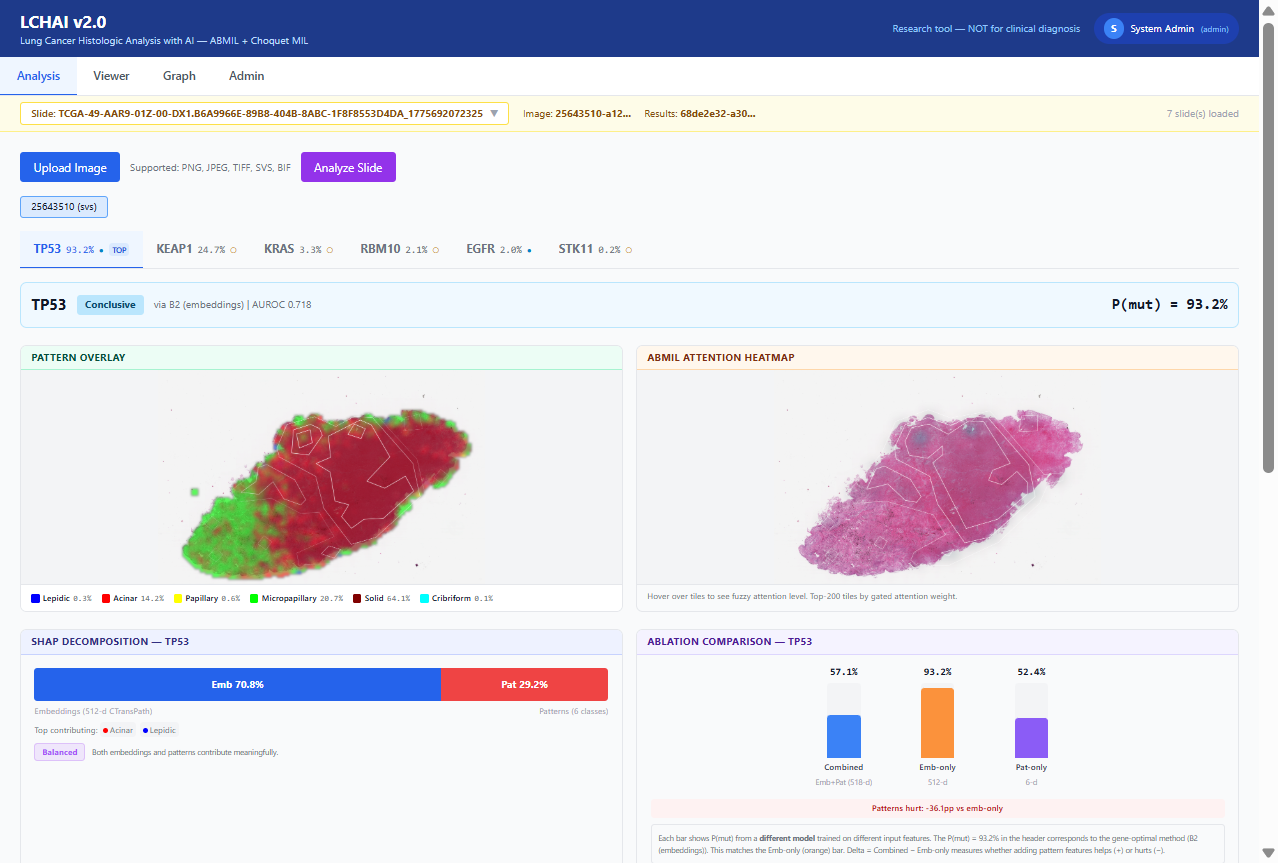
\includegraphics[width=\textwidth]{chapters/figures/lchai_v2_analysis_tab_overview.png}
\caption[LCHAI~v2.0 Analysis tab --- TP53 overview]{%
    LCHAI~v2.0 Analysis tab displaying results for TP53
    ($P(\text{mut}) = 93.2\%$, Conclusive).
    Gene sub-tabs sorted by descending $P(\text{mut})$ are shown
    at the top (TP53 selected as highest).
    \textbf{Top row}: Side-by-side pattern overlay (left) with
    composition percentages in the legend, and ABMIL attention
    heatmap (right) with interactive hover support.
    \textbf{Middle row}: SHAP decomposition with ``Balanced'' fuzzy
    label (left) and ablation comparison with model clarification
    text (right).}
\label{fig:lchai_v2_images}
\end{figure}

\begin{figure}[ht!]
\centering
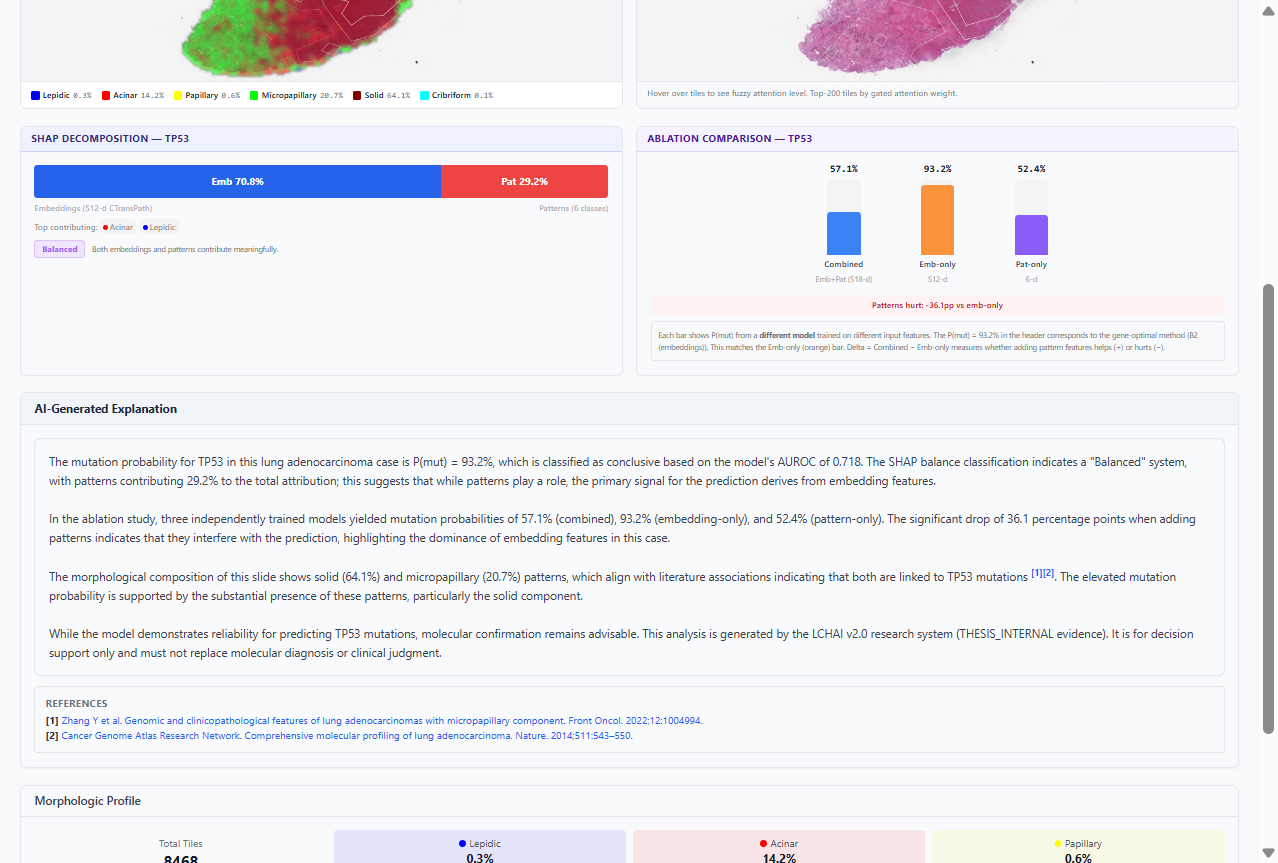
\includegraphics[width=\textwidth]{chapters/figures/lchai_v2_analysis_explanation.png}
\caption[LCHAI~v2.0 Analysis tab --- AI explanation with citations]{%
    AI-Generated Explanation for TP53 on the same slide.
    The explanation cites $P(\text{mut}) = 93.2\%$, the SHAP balance
    (``Balanced''), the ablation delta ($-36.1$\,pp), and
    literature-expected pattern associations with numbered PubMed
    references [1]~(Zhang et~al., 2022) and [2]~(TCGA, 2014)
    obtained from the knowledge graph.
    The ``REFERENCES'' section below provides clickable PubMed links.
    All fuzzy labels and clinical facts are system-controlled.}
\label{fig:lchai_v2_explanation}
\end{figure}

\subsubsection{Viewer Tab}
\label{sec:impl:lchai:ui:viewer}

The Viewer tab (Figure~\ref{fig:lchai_v2_viewer}) provides an
interactive whole-slide image viewer with four overlay modes selectable
via numbered buttons:
\begin{enumerate}
    \item \textbf{Original:} The unmodified H\&E-stained slide at full
    resolution, navigable via pan and zoom.
    \item \textbf{Patterns:} A tile-level colour overlay showing the
    predicted histological pattern for each tile (lepidic, acinar,
    papillary, micropapillary, solid, cribriform), with adjustable
    opacity.  The overlay is clipped to tissue regions to prevent
    colour bleeding onto the glass background.
    \item \textbf{Attention:} A heatmap of the ABMIL attention weights,
    highlighting tiles the model considers most informative for
    mutation prediction (blue = low attention, red = high attention).
    \item \textbf{Combined:} A merged view superimposing both pattern
    colours and attention intensity, enabling simultaneous assessment
    of \emph{what} the model sees and \emph{where} it attends.
\end{enumerate}
The viewer displays the dominant pattern name, total tile count, and
current zoom level in the header bar.
A colour legend at the bottom maps each pattern to its assigned colour.

\begin{figure}[ht!]
\centering
\begin{minipage}[t]{0.48\textwidth}
\centering
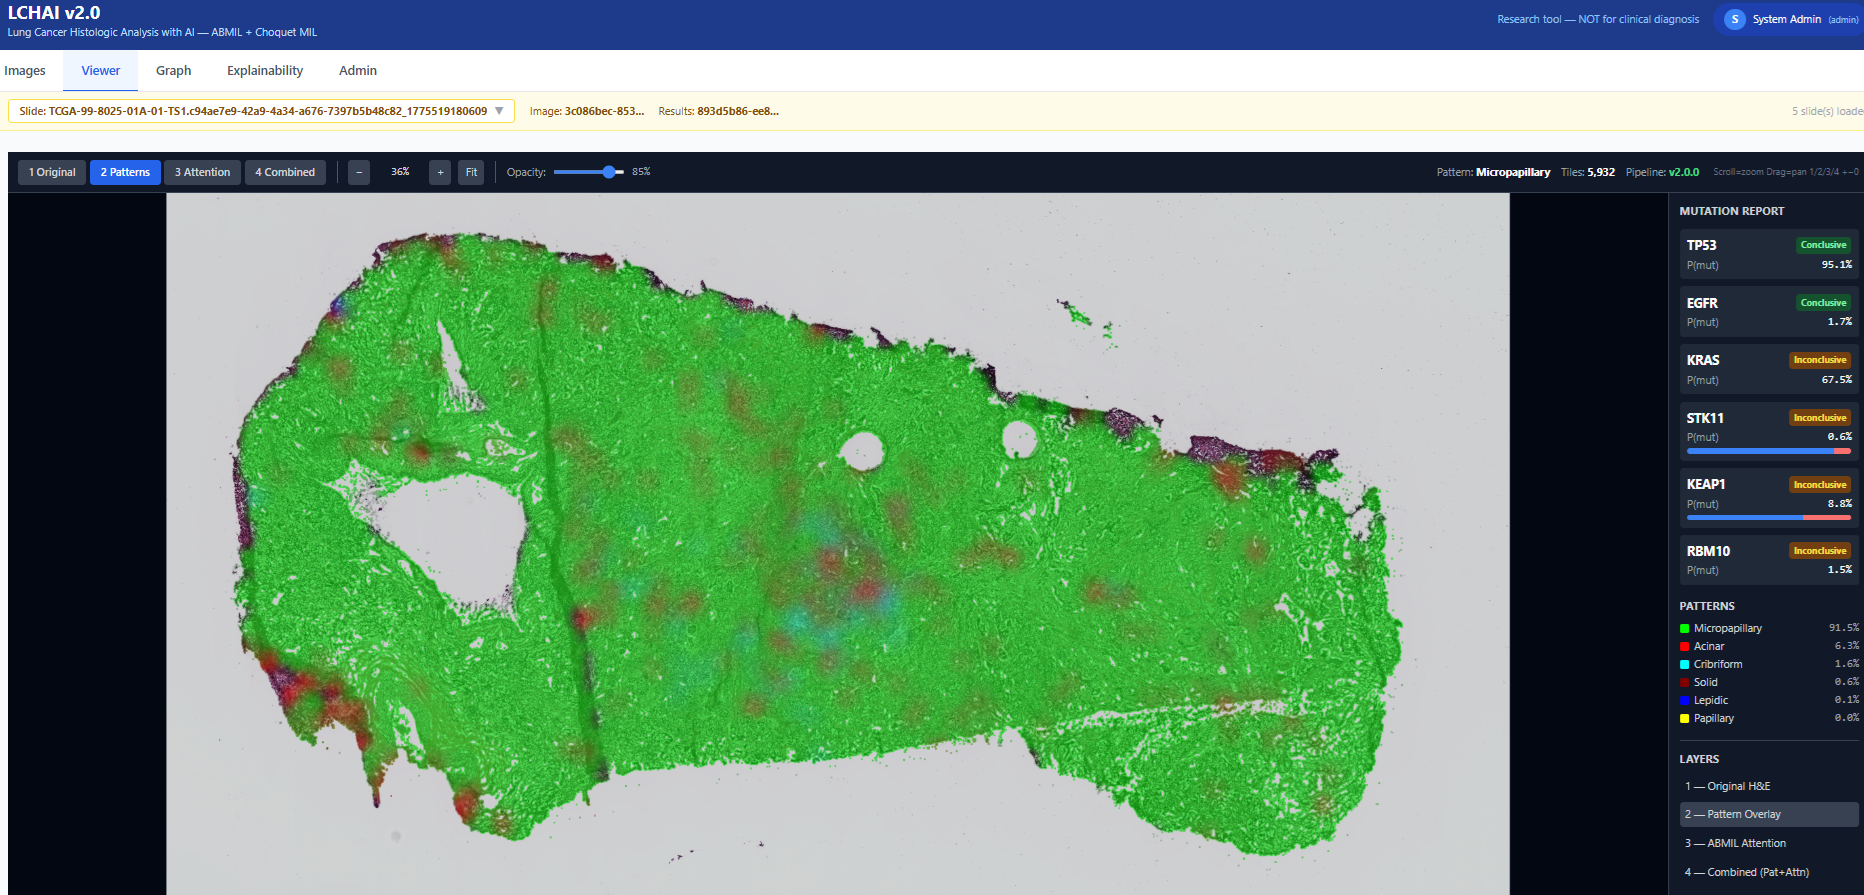
\includegraphics[width=\textwidth]{chapters/figures/lchai_v2_viewer_patterns_99_8025.png}
\end{minipage}\hfill
\begin{minipage}[t]{0.48\textwidth}
\centering
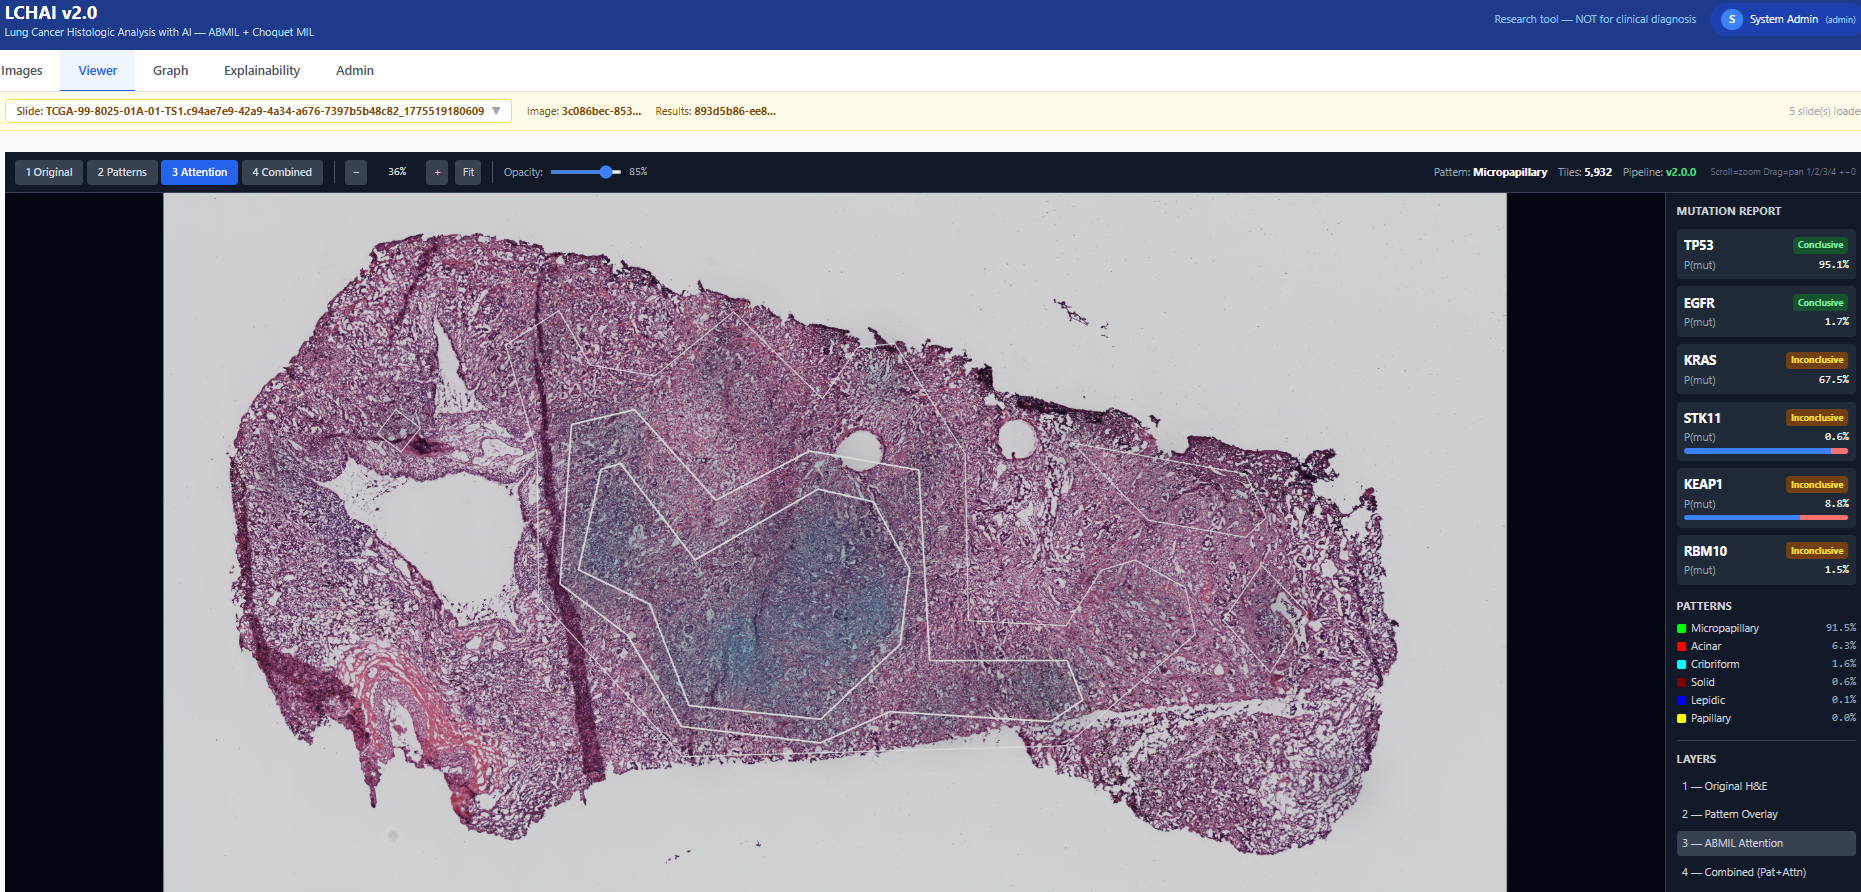
\includegraphics[width=\textwidth]{chapters/figures/lchai_v2_viewer_attention_99_8025.png}
\end{minipage}
\caption[LCHAI~v2.0 Viewer tab]{%
    LCHAI~v2.0 Viewer tab for case TCGA-99-8025.
    \textbf{Left}: Pattern overlay mode showing the tile-level categorical colour map
    with adjustable opacity (lepidic = blue, acinar = red, papillary = yellow,
    micropapillary = green, solid = dark red, cribriform = cyan).
    \textbf{Right}: ABMIL attention map mode showing attention-weight heatmap
    (blue = low, red = high attention).
    Both overlays are clipped to tissue regions; the user can pan, zoom, and
    toggle between all four modes (Original, Patterns, Attention, Combined).}
\label{fig:lchai_v2_viewer}
\end{figure}

\textbf{Active Learning: Pattern Correction Mode.}
The Viewer tab includes a built-in expert correction tool for the
active learning mechanism described in
Section~\ref{sec:meth:active_learning}.
Clicking ``Correct Patterns'' activates a lasso drawing mode: the
pathologist clicks and drags to draw a polygon over misclassified tiles.
All tiles whose centre falls within the polygon are selected
(highlighted in red, Figure~\ref{fig:lchai_v2_active_learning}).
The pathologist then selects the correct pattern from a dropdown of
the six ANORAK classes and clicks ``Save \& Retrain.''

The system submits the corrections to the \texttt{active-learning-service}
microservice, which:
\begin{enumerate}
    \item Persists corrections in the database with provenance metadata.
    \item Downloads the pre-computed tile embeddings
    (\texttt{tile\_data.npz}) from object storage.
    \item Runs delta training: head-only fine-tuning of the
    FuzzyArcLoss~V2 classification head for 10 epochs.
    \item Saves the updated model as a new version in MinIO.
    \item Re-runs the full inference pipeline with the corrected
    classifier, producing updated pattern overlays and mutation
    predictions.
\end{enumerate}

A real-time progress bar tracks the retraining status.
The pathologist can draw multiple lassos to accumulate corrections
before submitting, and the feedback loop allows further corrections
after reviewing the updated overlay.
Figure~\ref{fig:active_learning_workflow} illustrates the complete
workflow.

\begin{figure}[ht!]
\centering
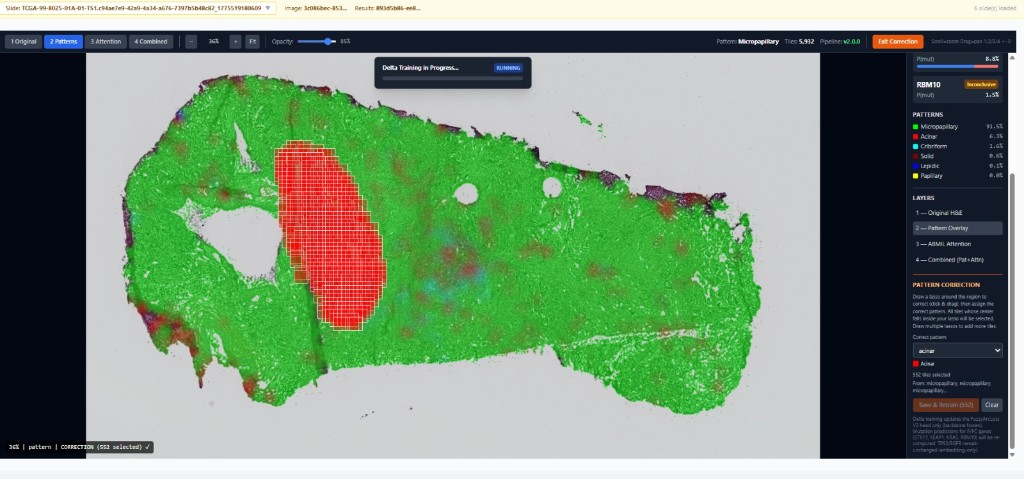
\includegraphics[width=\textwidth]{chapters/figures/lchai_v2_active_learning_correction.png}
\caption[LCHAI~v2.0 Viewer --- Active Learning correction mode]{%
    LCHAI~v2.0 Viewer tab in pattern correction mode.
    The pathologist has drawn a lasso around 152 micropapillary-classified
    tiles and selected ``acinar'' as the correct pattern.
    Selected tiles are highlighted in red.
    The sidebar shows the correction panel with pattern dropdown,
    tile count, and ``Save \& Retrain'' button.
    A ``Delta Training in Progress'' indicator is visible at the top.}
\label{fig:lchai_v2_active_learning}
\end{figure}

\begin{figure}[ht!]
\centering
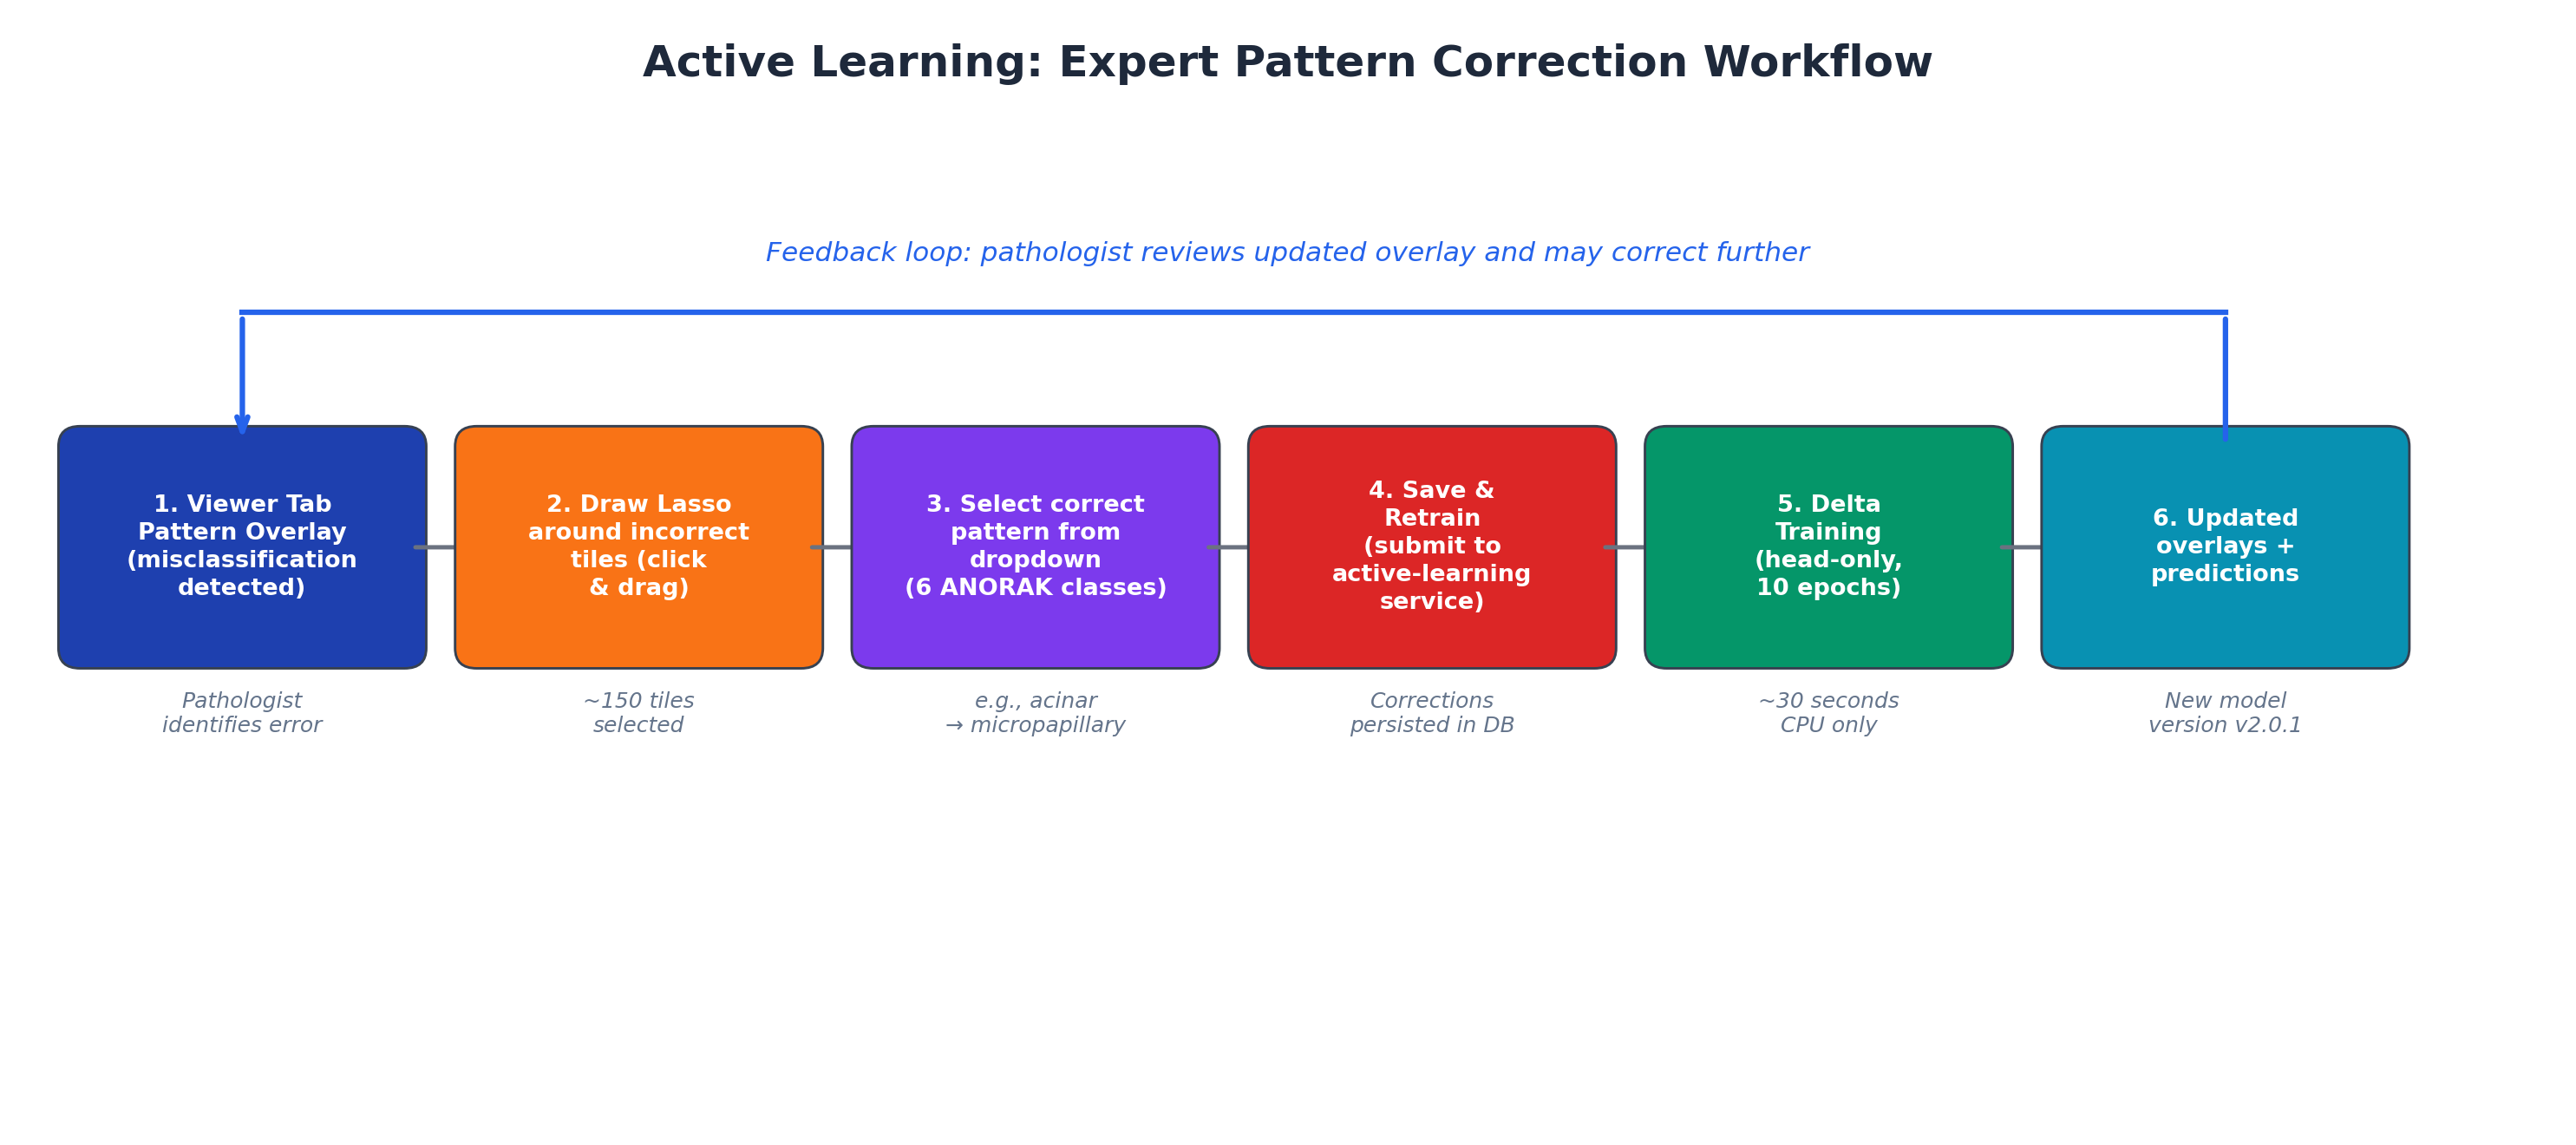
\includegraphics[width=\textwidth]{chapters/figures/active_learning_workflow.png}
\caption[Active Learning correction workflow]{%
    Active Learning expert correction workflow.
    The pathologist (1)~identifies misclassified tiles in the pattern
    overlay, (2)~draws a lasso to select them, (3)~assigns the correct
    pattern, (4)~submits corrections, (5)~delta training runs
    ($\sim$30 seconds, head-only), and (6)~updated overlays and
    mutation predictions are displayed.
    The feedback loop allows iterative refinement.}
\label{fig:active_learning_workflow}
\end{figure}

\subsubsection{Graph Tab}
\label{sec:impl:lchai:ui:graph}

The Graph tab (Figure~\ref{fig:lchai_v2_graph}) displays an interactive
force-directed knowledge graph dynamically constructed from the case's
inference results and the curated ontology layer
(Section~\ref{sec:impl:ontology}).
Nodes are colour-coded by entity type: blue~= case, red~= gene,
orange~= pattern, green~= diagnosis, cyan~= stage,
dark red~= mutation, purple~= treatment, and grey~= ontology reference.
Edges are drawn as solid lines (asserted/curated relations) or dashed
lines (inferred relations from the DeepSearch pipeline).

A ``Rebuild Graph'' button triggers re-computation of the case-specific
subgraph, and an ``Explain with AI'' button invokes the LLM explanation
agent (Section~\ref{sec:impl:ontology:llm}) to produce a
natural-language narrative displayed below the graph
(Figure~\ref{fig:lchai_v2_graph_explain}).  The explanation
summarises the detected histological patterns, predicted mutations,
treatment options, and relevant disclaimers.

\begin{figure}[ht!]
\centering
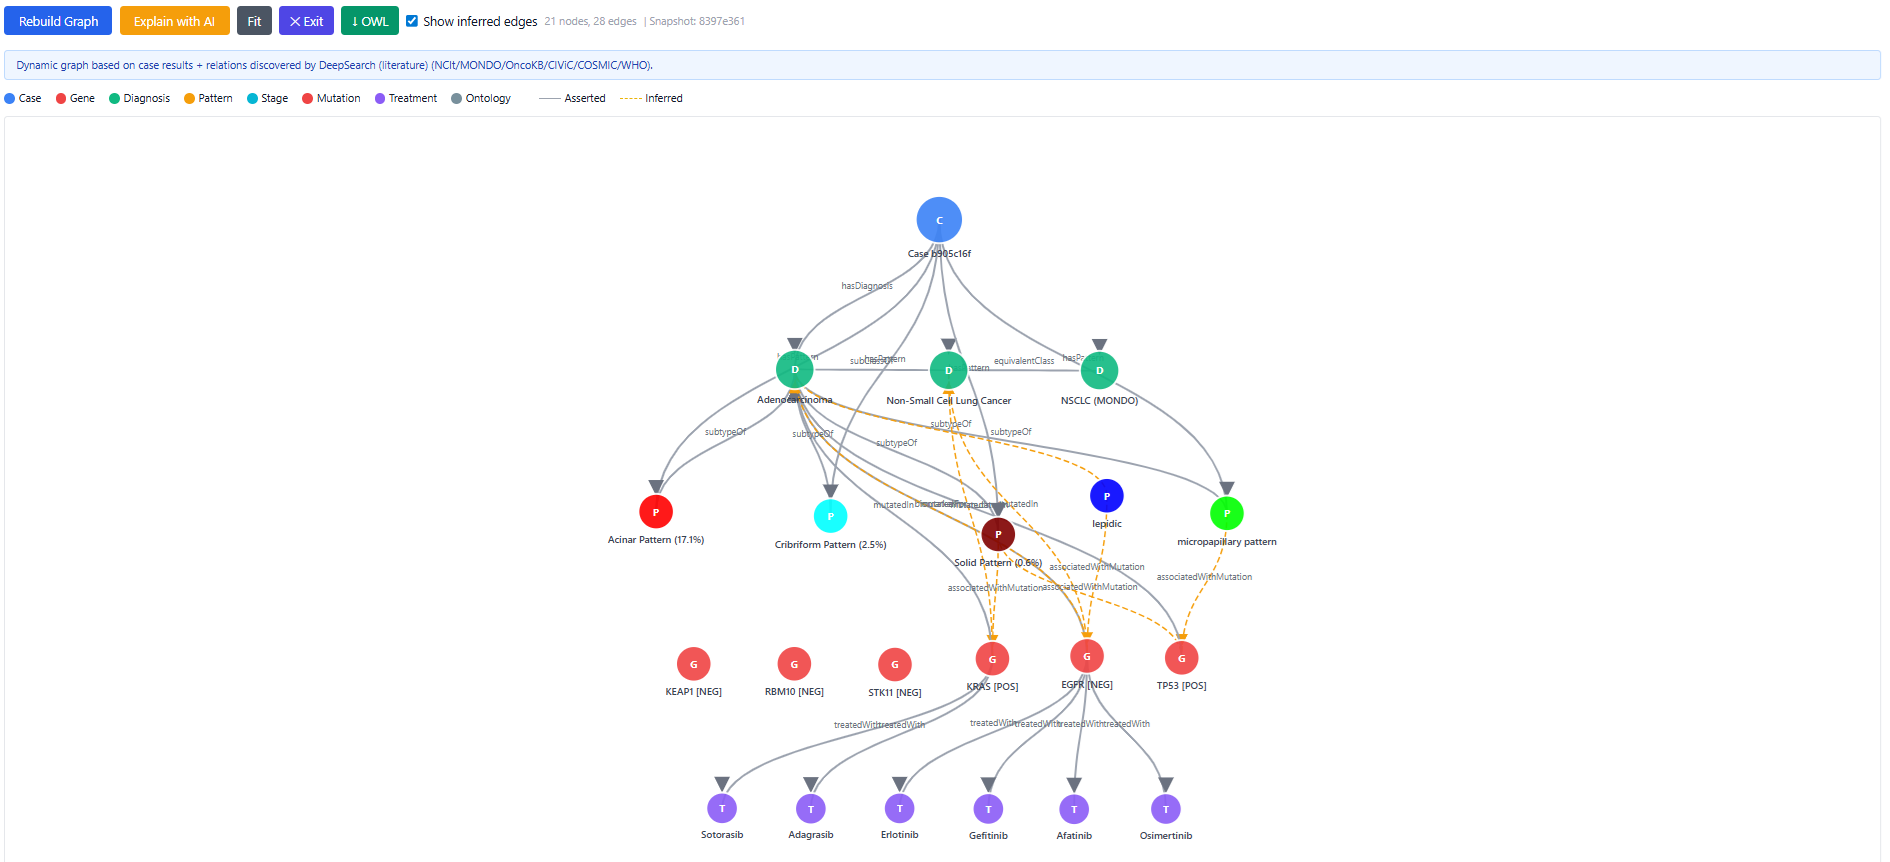
\includegraphics[width=\textwidth]{chapters/figures/lchai_v2_graph_tab_55_7815.png}
\caption[LCHAI~v2.0 Graph tab]{%
    LCHAI~v2.0 Graph tab displaying the hierarchical knowledge graph for case
    TCGA-55-7815.  The graph is organized in layers: Case (top, blue) $\to$
    Patterns (orange) $\to$ Diagnosis (green) $\to$ Genes (red) $\to$
    Treatments (purple).  Solid lines represent asserted/curated relations;
    dashed lines represent inferred relations from the DeepSearch pipeline.
    KRAS [POS] and TP53 [POS] are linked to their respective targeted therapies
    (sotorasib, adagrasib for KRAS; checkpoint-related for TP53).
    The graph can be exported in OWL/RDF format for downstream ontological analysis.}
\label{fig:lchai_v2_graph}
\end{figure}

\begin{figure}[ht!]
\centering
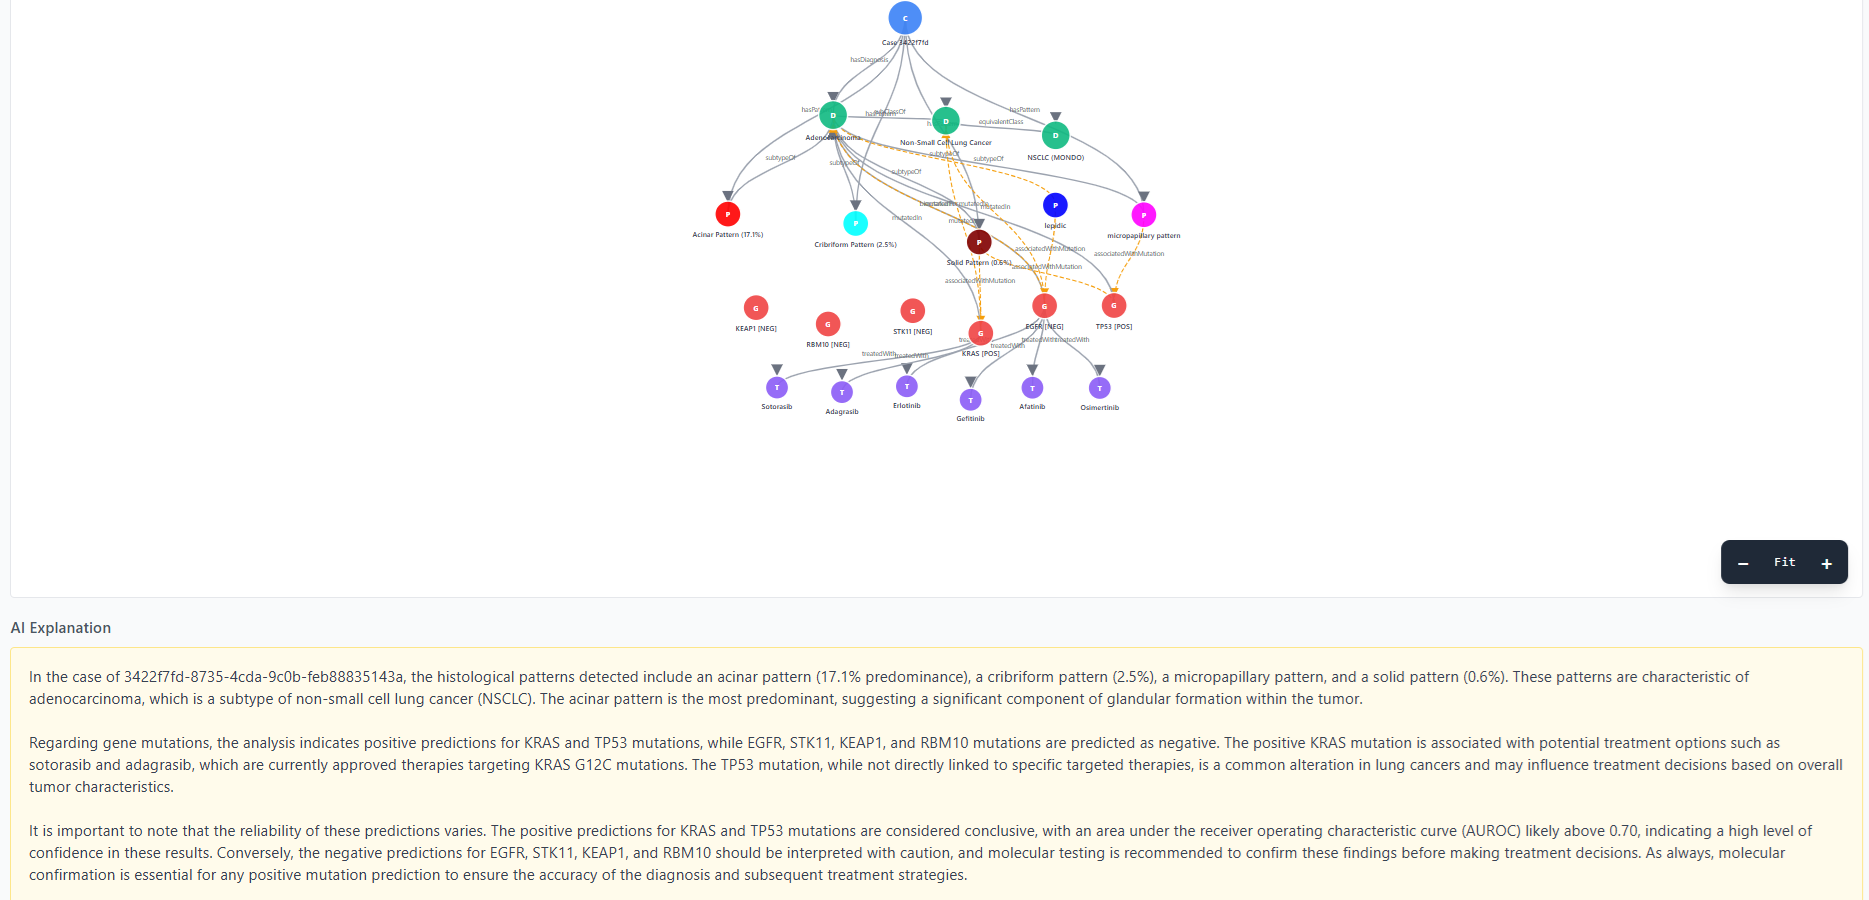
\includegraphics[width=\textwidth]{chapters/figures/lchai_v2_graph_explain_ai.png}
\caption[LCHAI~v2.0 Graph --- LLM explanation]{%
    LLM-generated natural language explanation for the case-specific knowledge
    graph.  The explanation summarises the detected histological patterns,
    predicted mutations, associated treatment options, and relevant clinical
    disclaimers.  The narrative is generated by GPT-4o-mini using the graph
    structure as context.}
\label{fig:lchai_v2_graph_explain}
\end{figure}

\subsubsection{Fuzzy Linguistic Labels for XAI Outputs}
\label{sec:impl:lchai:fuzzy_labels}

Numeric XAI outputs---SHAP percentages, Choquet Shapley values,
interaction indices, and attention weights---are difficult for clinicians
to interpret without a reference scale.
LCHAI~v2.0 addresses this by applying \emph{fuzzy linguistic labels}:
trapezoidal membership functions (Section~\ref{sec:bg:fuzzy:sets}) that
map continuous numeric values to human-readable intensity terms.
Five fuzzy scales are defined:
(1)~\textbf{SHAP Balance} (Embedding-Dominated to Pattern-Dominated);
(2)~\textbf{Shapley Profile} (Uniform to Highly Polarised);
(3)~\textbf{Shapley Individual} (Average to Strongly Above/Below);
(4)~\textbf{Interaction Index} (Negligible to Very Strong, with Synergy/Redundancy direction);
(5)~\textbf{ABMIL Attention Level} (Very Low to Very High Attention).
All thresholds are configurable via the Admin~$\to$~Fuzzy Labels panel.

\textbf{Anti-hallucination mechanism.}
The fuzzy labels are computed deterministically by the system and injected
verbatim into the LLM prompt with an explicit instruction:
``Use these exact labels. Do NOT invent different intensity words.''
Combined with the knowledge graph grounding of clinical associations,
this creates a dual anti-hallucination layer: the KG constrains \emph{what}
the LLM says (clinical facts), and the fuzzy labels constrain \emph{how}
it says it (intensity and directionality).

\textbf{Fourth level of fuzzy logic.}
This extends the coherent application of fuzzy logic to a fourth level:
(i)~training (FuzzyArcLoss~V2), (ii)~representation (soft probabilities),
(iii)~aggregation (Choquet integral), and (iv)~interpretation (fuzzy
linguistic labels on XAI outputs).

\begin{figure}[ht!]
\centering
\begin{minipage}[t]{0.48\textwidth}
\centering
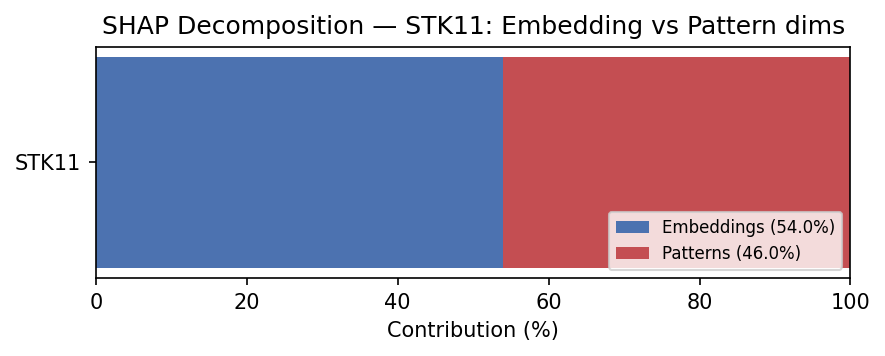
\includegraphics[width=\textwidth]{chapters/figures/shap_decomp_STK11_55_7815_bar.png}
\end{minipage}\hfill
\begin{minipage}[t]{0.48\textwidth}
\centering
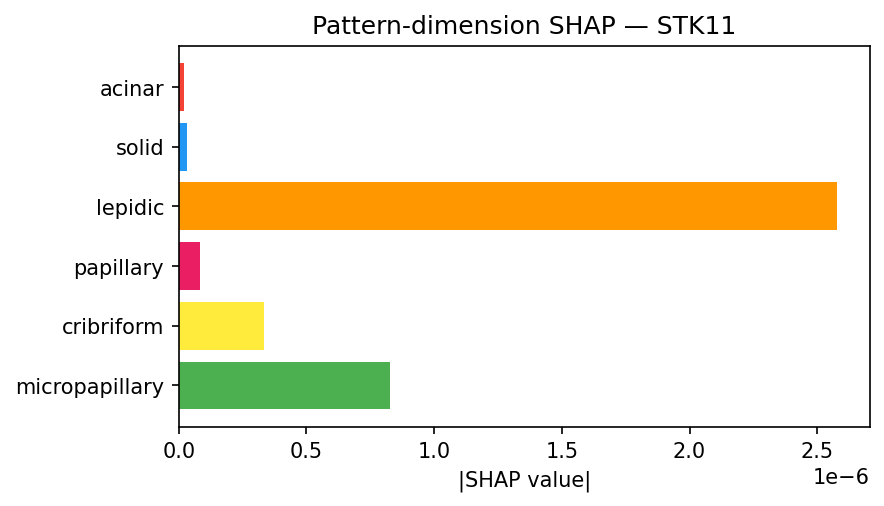
\includegraphics[width=\textwidth]{chapters/figures/shap_decomp_STK11_55_7815_patterns.png}
\end{minipage}
\caption[LCHAI~v2.0 SHAP Decomposition --- STK11]{%
    SHAP decomposition for STK11 (PI-ABMIL method) on
    TCGA-55-7815 (P(mut)~$= 0.5\%$, Inconclusive).
    \textbf{Left}: Embedding vs.\ pattern contribution stacked bar.
    Embeddings contribute 51\% and patterns 49\% of the SHAP
    attribution.
    Note that SHAP attribution reflects how the model distributes
    attention, not necessarily positive contribution (see
    Section~\ref{sec:eval:interp:enrichment} for ablation evidence).
    \textbf{Right}: Pattern-dimension SHAP values showing the
    absolute contribution of each histological pattern.
    Lepidic has the highest $|$SHAP$|$ value, followed by
    micropapillary and cribriform.
    STK11 is associated with a variable, immune-cold microenvironment~\cite{skoulidis2018stk11immune}; the diffuse SHAP distribution across patterns
    is consistent with this characterisation.}
\label{fig:lchai_v2_shap_decomp}
\end{figure}

% Old Output 4 text removed — Choquet description is now in the Analysis Tab section above.

\begin{figure}[ht!]
\centering
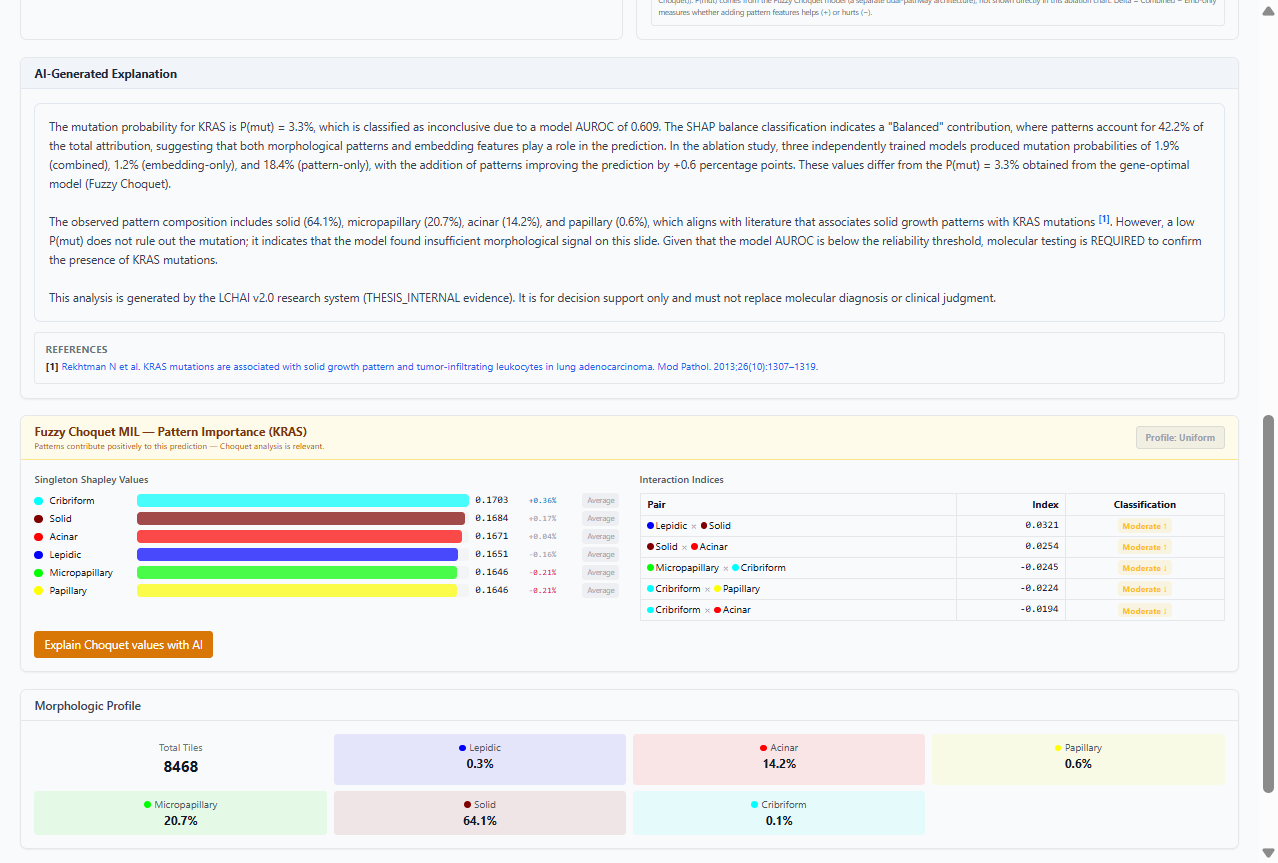
\includegraphics[width=\textwidth]{chapters/figures/lchai_v2_analysis_choquet_fuzzy.png}
\caption[LCHAI~v2.0 Analysis --- Choquet Shapley with fuzzy labels]{%
    Analysis tab for KRAS (Inconclusive, 3.3\%) showing the
    AI-generated explanation, references, and the conditional Fuzzy
    Choquet MIL panel (displayed because patterns contribute
    positively for KRAS).
    \textbf{Choquet panel}: ``Profile: Uniform'' badge indicates
    near-uniform Shapley values; per-pattern bars show individual
    fuzzy labels (``Average''); the interaction index table classifies
    each pair (e.g., ``Moderate Synergy~$\uparrow$'' for
    lepidic$\times$solid at $+0.032$).
    The morphologic profile at the bottom shows the six-pattern
    composition of the slide.}
\label{fig:lchai_v2_choquet}
\end{figure}

\subsubsection{Admin Tab}
\label{sec:impl:lchai:ui:admin}

The Admin tab (accessible only to users with the \texttt{admin} role)
provides seven sub-tabs:

\begin{enumerate}
    \item \textbf{Parameters:} Adjustable inference parameters including
    the AUROC conclusive threshold, maximum tiles per WSI, and
    permutation analysis repeats
    (Figure~\ref{fig:lchai_v2_admin_params}).

    \item \textbf{DeepSearch Pipeline:} Interface for running the
    relation-discovery pipeline (Section~\ref{sec:impl:ontology:deepsearch})
    on free-text input or batch literature queries.

    \item \textbf{Reference:} Clinical reference tables for mutation
    probability interpretation ranges.

    \item \textbf{KG Versions:} Knowledge graph snapshot management with
    versioned changelogs.

    \item \textbf{Ontology Management:} Interface for creating ontology
    update proposals and reviewing discovered relations.

    \item \textbf{Audit Log:} A chronological log of all system events
    (image uploads, inference completions) recording the authenticated
    user, case identifier, action type, and timestamp
    (Figure~\ref{fig:lchai_v2_audit}).

    \item \textbf{Fuzzy Labels:} An editor for the five trapezoidal
    membership function scales used to classify XAI outputs
    (Section~\ref{sec:impl:lchai:fuzzy_labels}).
    Each scale displays editable rows (label, colour, trapezoidal
    corners $[a,b,c,d]$) with a real-time SVG preview, enabling domain
    experts to calibrate linguistic boundaries without code changes.
\end{enumerate}

\begin{figure}[ht!]
\centering
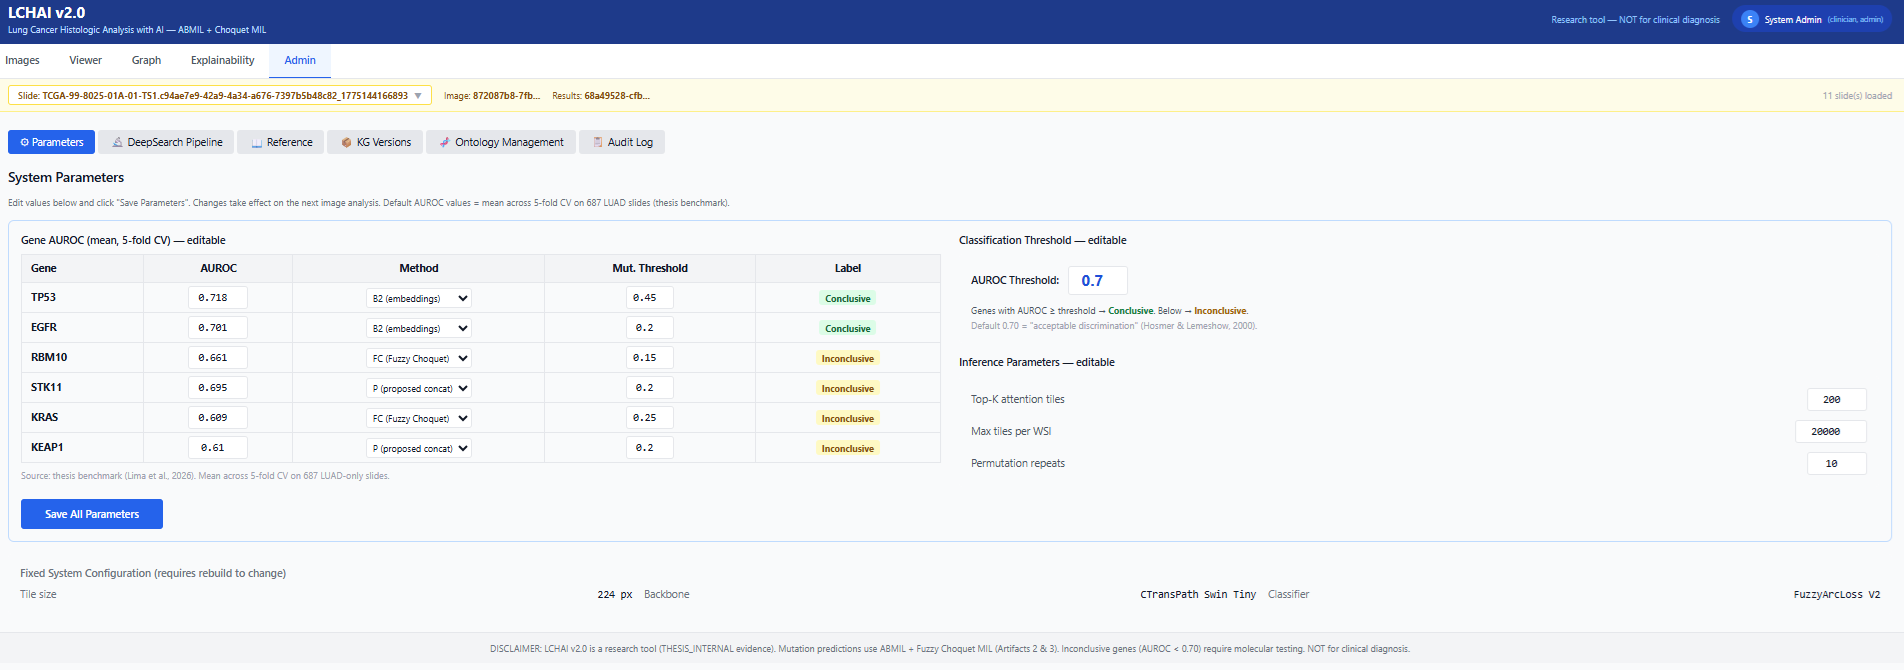
\includegraphics[width=\textwidth]{chapters/figures/lchai_v2_admin_params.png}
\caption[LCHAI~v2.0 Admin --- System Parameters]{%
    System Parameters sub-tab in the Admin panel.  Adjustable per-gene AUROC
    thresholds, prediction method selection (B2/PI-ABMIL/FC-MIL), and inference parameters
    (classification threshold, min/max tiles).  Default AUROC values are the
    mean across 5-fold CV on 687 LUAD slides.}
\label{fig:lchai_v2_admin_params}
\end{figure}

\begin{figure}[ht!]
\centering
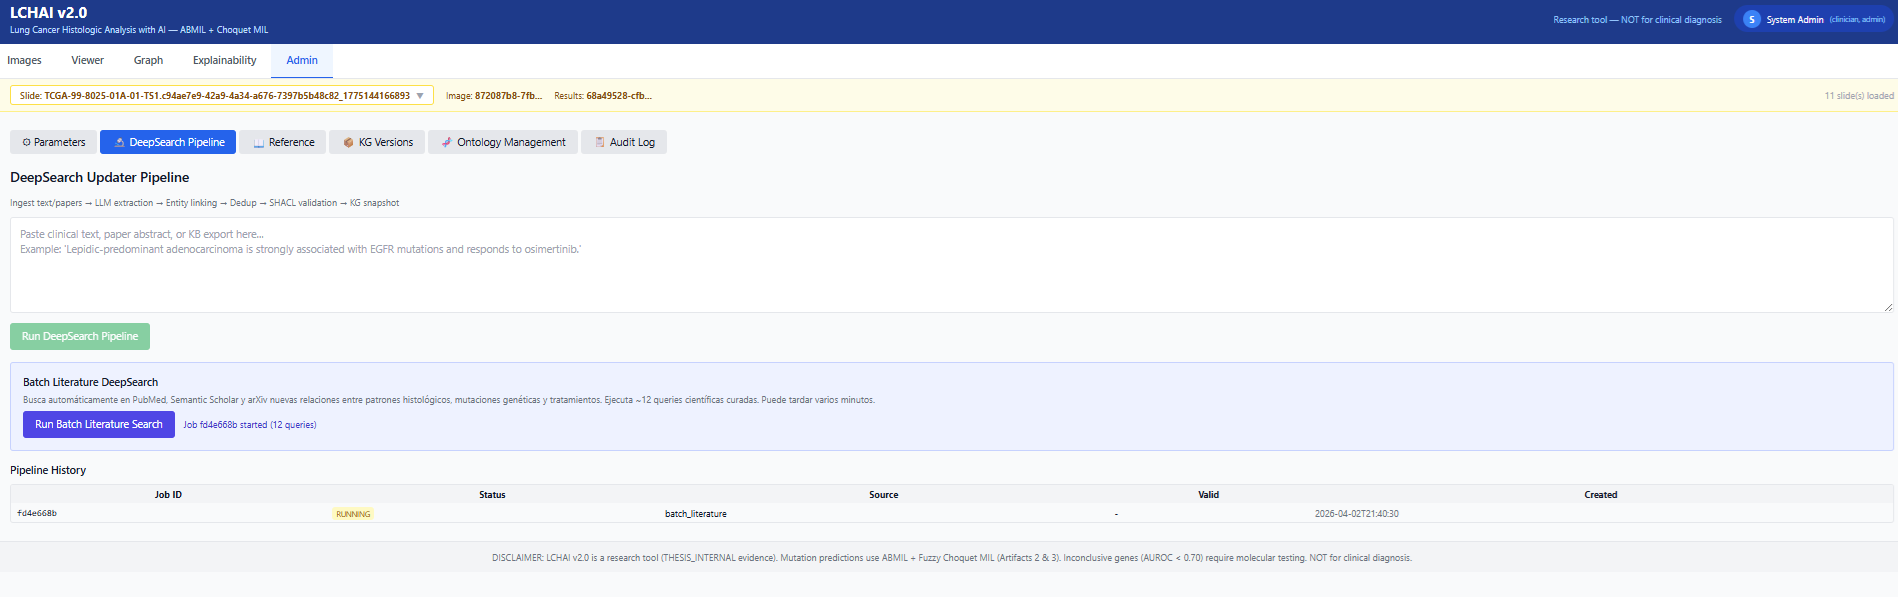
\includegraphics[width=\textwidth]{chapters/figures/lchai_v2_admin_audit_new.png}
\caption[LCHAI~v2.0 Admin --- Audit Log]{%
    Audit Log sub-tab in the Admin panel.  Each event records the
    authenticated user, event type (\texttt{image.uploaded}),
    case identifier, filename, and UTC timestamp.
    Events are published via RabbitMQ and persisted by the
    audit-service consumer.}
\label{fig:lchai_v2_audit}
\end{figure}

\section{Implementation of the Ontology Explanation Layer}
\label{sec:impl:ontology}
 
This section describes the software implementation of the multi-ontology
knowledge graph and explanation layer that addresses RQ6 and RQ7.
 
\subsection{Knowledge Graph Construction}
\label{sec:impl:ontology:construction}

The knowledge graph is constructed as a \emph{curated edge store}
rather than by parsing complete OWL ontology files.
Each entity (pattern, gene, diagnosis, treatment) is identified by
its canonical IRI from the NCI Thesaurus (NCIt) or MONDO Disease
Ontology, and each relationship edge carries a \texttt{provenance}
attribute citing the specific evidence source.

Table~\ref{tab:kg_curated_edges} summarises the curated pattern--gene
edges and their literature provenance.
The full knowledge base contains 30 curated edges across five
relationship types:

\begin{itemize}
    \item \texttt{subtypeOf}: histological patterns as subtypes of
    adenocarcinoma (WHO 2021~\cite{who2021thoracic})
    \item \texttt{associatedWithMutation}: pattern--gene morphology-molecular
    correlations, each backed by a specific PubMed citation
    \item \texttt{treatedWith}: gene--drug therapeutic relations
    (OncoKB/FDA-approved)
    \item \texttt{mutatedIn}: gene--diagnosis relations (COSMIC)
    \item \texttt{equivalentClass}: cross-ontology mapping
    (NCIt $\leftrightarrow$ MONDO)
\end{itemize}

\begin{table}[ht!]
\centering
\caption[Curated pattern--gene edges with literature provenance]{%
    Curated \texttt{associatedWithMutation} edges in the knowledge
    graph.  Each edge links a histological growth pattern to a driver
    gene based on published morphology--molecular correlation studies.
    Patterns without established gene associations (acinar, cribriform)
    have no edges.}
\label{tab:kg_curated_edges}
\small
\begin{tabular}{l l l l}
\hline
\textbf{Pattern} & \textbf{Gene} & \textbf{Evidence} & \textbf{PMID} \\
\hline
Lepidic & EGFR & 90.5\% EGFR in lepidic (2017) & 27738759 \\
Papillary & EGFR & EGFR-enriched intermediate (2011) & 21252858 \\
Micropapillary & TP53 & TP53 57.4\% in micropap. LUAD (2022) & 36457500 \\
Micropapillary & ALK & ALK+ in micropap. histology (2011) & 21753699 \\
Solid & KRAS & Solid 27\% in KRAS+ (2013) & 23619604 \\
Solid & TP53 & TP53 high-grade assoc. (TCGA 2014) & 25079552 \\
\hline
Acinar & --- & No enrichment (pooled OR 0.65 KRAS) & --- \\
Cribriform & --- & Rare; no established association & --- \\
\hline
\end{tabular}
\end{table}
 
\subsection{Three-Layer Runtime Architecture}
\label{sec:impl:ontology:runtime}
 
At inference time, the knowledge graph operates through three layers
(Figure~\ref{fig:kg_layers}):
 
\textbf{Layer~1 (Curated):} 30 hand-curated edges grounded in
WHO 2021, OncoKB/FDA, and peer-reviewed literature (with specific
PMIDs as provenance --- see Table~\ref{tab:kg_curated_edges}).
This layer is static and version-controlled.
 
\textbf{Layer~2 (Dynamic case filter):} the system queries the case's
inference results and retains only the subgraph relevant to its pattern
composition and mutation predictions.
Nodes with no connection to the case are suppressed.
 
\textbf{Layer~3 (DeepSearch-discovered):} periodically enriched by the
batch pipeline described in Section~\ref{sec:impl:ontology:deepsearch}.
 
\begin{figure}[H]
\centering

\includegraphics[width=\textwidth]{chapters/figures/kg_three_layer_architecture.png}
\caption[Three-layer knowledge graph architecture]{%
    Three-layer knowledge graph architecture.
    \textbf{Layer~1} (top): curated assertions from WHO, OncoKB/FDA,
    TCGA/CIViC, and COSMIC with provenance annotations.
    \textbf{Layer~2} (middle): dynamic case filtering for
    TCGA-55-7815 (micropapillary 79.4\%, acinar 17.1\%); only TP53 and KRAS
    and their therapies (sotorasib for KRAS) are retained; TP53 has
    no targeted therapy.
    \textbf{Layer~3} (bottom): DeepSearch pipeline ingesting PubMed,
    Semantic Scholar, and arXiv abstracts, extracting relation triples
    via LLM, and merging validated edges as \texttt{inferred} relations.}

\label{fig:kg_layers}
\end{figure}
 
\subsection{Dynamic Case Graph}
\label{sec:impl:ontology:case_graph}

The rendered case graph for TCGA-55-7815 is shown in
Figure~\ref{fig:lchai_v2_graph} (Section~\ref{sec:impl:lchai:ui:graph}).
The graph contains 22 nodes and 31 edges (30 curated + 1 DeepSearch-discovered),
dynamically assembled from the curated knowledge base and active
discovered relations based on the case's pattern composition
(micropapillary-predominant, 79.4\%) and mutation predictions
(KRAS [POS] and TP53 [POS]).
The hierarchical layout---Case $\to$ Patterns $\to$ Diagnosis $\to$
Genes $\to$ Treatments---makes the clinical reasoning chain visually
explicit.
Solid edges represent curated relations (WHO, OncoKB);
dashed edges represent inferred morphology--molecular correlations
(each with a PMID) and relations discovered by the
DeepSearch pipeline (Section~\ref{sec:impl:ontology:deepsearch}).
The graph is exportable in OWL/RDF format for downstream ontological
analysis.
\textbf{KPI~6:} the dynamic case graph with typed entities and
provenance categories is demonstrated.
 
\subsection{DeepSearch Enrichment Pipeline}
\label{sec:impl:ontology:deepsearch}
 
The \texttt{DeepSearchUpdater} pipeline discovers new
pattern--gene--treatment relationships from the scientific literature
and incorporates them into the knowledge graph as Layer~3 edges.
The pipeline operates in six stages:

\begin{enumerate}
    \item \textbf{Batch literature search.}
    Twelve curated queries (Table~\ref{tab:deepsearch_queries}) are
    dispatched against three databases: PubMed (NCBI E-utilities API),
    Semantic Scholar (Graph API), and arXiv (OAI API).
    Up to five papers per source per query are retrieved, yielding up
    to $12 \times 3 \times 5 = 180$ candidate abstracts per batch run.

\begin{table}[ht!]
\centering
\small
\caption{The 12 curated DeepSearch queries used for batch literature
search.  Queries are grouped by topic: pattern--mutation associations
(Q1--Q3), treatment--mutation relationships (Q4--Q10), and emerging
biomarkers and methods (Q11--Q12).}
\label{tab:deepsearch_queries}
\begin{tabular}{c l}
\hline
\textbf{ID} & \textbf{Query string} \\
\hline
Q1  & lung adenocarcinoma histologic pattern EGFR KRAS mutation association \\
Q2  & lepidic acinar papillary micropapillary solid pattern lung cancer prognosis \\
Q3  & lung adenocarcinoma morphology molecular subtypes targetable mutations \\
Q4  & EGFR mutant NSCLC targeted therapy osimertinib resistance \\
Q5  & KRAS G12C lung cancer sotorasib adagrasib clinical trial \\
Q6  & ALK rearrangement NSCLC alectinib lorlatinib treatment \\
Q7  & BRAF V600E lung adenocarcinoma dabrafenib trametinib \\
Q8  & RET fusion NSCLC selpercatinib pralsetinib \\
Q9  & MET exon 14 skipping lung cancer capmatinib tepotinib \\
Q10 & HER2 ERBB2 NSCLC trastuzumab deruxtecan \\
Q11 & NSCLC immunotherapy biomarker PD-L1 TMB \\
Q12 & lung cancer histopathology deep learning mutation prediction \\
\hline
\end{tabular}
\end{table}

    \item \textbf{LLM relation extraction.}
    Each abstract is processed by an LLM (OpenAI GPT-4o-mini) with a
    structured prompt that constrains output to JSON triples of the
    form \texttt{(subject, predicate, object, evidence\_quote)}.
    Allowed predicates are restricted to six domain-specific
    relationships: \texttt{associatedWithMutation},
    \texttt{treatedWith}, \texttt{subtypeOf}, \texttt{mutatedIn},
    \texttt{resistantTo}, and \texttt{biomarkerFor}.

    \item \textbf{Entity linking.}
    Extracted entity names (e.g., ``KRAS'', ``solid pattern'') are
    mapped to canonical ontology IRIs via a curated dictionary
    (\texttt{ENTITY\_IRI\_MAP}) covering all genes, patterns,
    diagnoses, and treatments in the knowledge base.
    Unresolved entities are discarded.

    \item \textbf{Deduplication.}
    Triples with identical \texttt{(subject\_iri, predicate,
    object\_iri)} from multiple papers are merged, preserving all
    source citations.

    \item \textbf{Type-constraint validation.}
    Rules analogous to SHACL shapes enforce type compatibility:
    \texttt{associatedWithMutation} requires a \emph{pattern}
    subject and a \emph{gene} object;
    \texttt{treatedWith} requires a \emph{gene} subject and a
    \emph{treatment} object.
    Triples violating these constraints are rejected.

    \item \textbf{Versioned persistence.}
    Valid relations are stored in the \texttt{discovered\_relations}
    table with metadata: paper source (PubMed/Semantic Scholar/arXiv),
    paper ID, evidence quote, and \texttt{is\_active} flag.
    A full changelog tracks additions, modifications, and
    deactivations.
\end{enumerate}

\paragraph{Graph integration.}
When the clinician clicks ``Rebuild Graph'' in the Graph tab, the
system merges Layer~1 curated edges with all \texttt{is\_active = true}
discovered relations from Layer~3.
Discovered edges appear as dashed orange arrows in the graph
visualisation, distinguished from solid grey curated edges.
Hovering over any edge displays its provenance (PMID or paper source).

\paragraph{False positive mitigation.}
LLM-extracted relations may contain false positives---for example,
a paper mentioning ``acinar'' and ``KRAS'' in the same abstract
does not necessarily imply a positive association (pooled evidence
actually shows an inverse relationship, OR~$= 0.65$,
$p < 0.01$~\cite{ejso2019pooled}).
Discovered relations can be individually deactivated by an
administrator via the ``Discovered Relations'' panel, setting
\texttt{is\_active = false} without deleting the record.
This preserves the audit trail while preventing incorrect edges
from appearing in the case graph.
 
\begin{figure}[ht!]
\centering
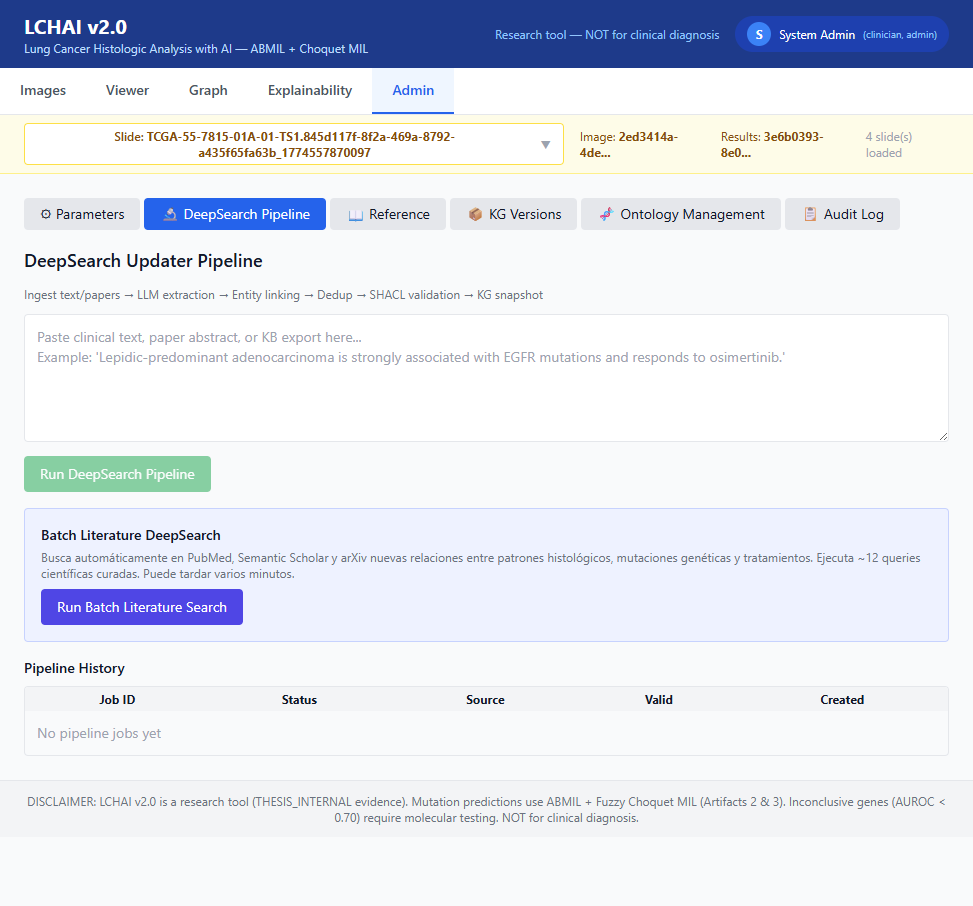
\includegraphics[width=\textwidth]{chapters/figures/lchai_v2_admin_deepsearch.png}
\caption[DeepSearch admin interface (v2.0)]{%
    DeepSearch batch pipeline interface in the LCHAI~v2.0 Admin panel.
    The ``Run DeepSearch Pipeline'' button accepts free-text input for
    single-query relation extraction via LLM.
    The ``Run Batch Literature Search'' button launches 12 curated
    queries across PubMed, Semantic Scholar, and arXiv.
    Pipeline History shows executed jobs with status, source type,
    validation results, and creation timestamp.
    \textbf{KPI~7:} validated discovered relations with provenance
    pointers are demonstrated.}
\label{fig:deepsearch_ui}
\end{figure}
 
\subsection{LLM-Based Natural Language Explanation}
\label{sec:impl:ontology:llm}

Beyond the structured graph, an explanation agent generates
natural-language summaries from the case graph's node and edge lists.
The agent supports multiple LLM backends (OpenAI GPT-4o-mini, Anthropic
Claude~3.5 Haiku) selectable via the \texttt{LLM\_PROVIDER} environment
variable, and includes clinical guardrails that prevent
prohibited phrases such as ``definitive diagnosis'' or ``confirmed
diagnosis,'' ensuring outputs remain within the system's intended scope
as a research and decision-support tool.

A critical design decision is that \textbf{every LLM explanation
is grounded in the current state of the knowledge graph}, not in
hardcoded clinical associations.
Before generating any explanation, the backend retrieves the
case-specific subgraph (curated edges + DeepSearch-discovered
relations) and injects its nodes and edges into the LLM prompt
as structured context.
The prompt explicitly instructs the LLM:

\begin{quote}
\emph{``Use ONLY these knowledge graph edges for pattern--gene and
gene--treatment associations.
Do NOT invent associations not present in this graph.''}
\end{quote}

This architecture ensures two properties:
\begin{enumerate}
    \item \textbf{Dual anti-hallucination grounding:} The LLM cannot
    fabricate clinical associations because its factual context is
    constrained to verified KG edges with provenance (PMIDs).
    Additionally, all intensity terms are computed by the fuzzy
    linguistic label system (Section~\ref{sec:impl:lchai:fuzzy_labels})
    and injected verbatim into the prompt.
    \item \textbf{Dynamic updating:} When DeepSearch discovers new
    relations (e.g., a newly published pattern--mutation association),
    these are automatically included in the KG context of subsequent
    explanations without any code changes.
    The number and content of pattern--gene associations evolve as the
    KG grows.
\end{enumerate}

The frontend also queries a dedicated endpoint
(\texttt{GET /graph/gene-associations}) that returns the full set of
curated and discovered pattern--gene and gene--treatment edges,
ensuring that all UI components display associations consistent with
the current KG state.

Two distinct LLM explanation modes are implemented:

\textbf{Graph-level explanation} (Graph tab, ``Explain with AI'' button):
generates a holistic case narrative from the knowledge graph's node and
edge lists, covering detected patterns, predicted mutations, treatment
options, and clinical disclaimers.
The full graph context is always injected.

\textbf{Gene-level explanation} (Analysis tab):
generates a per-gene narrative integrating the SHAP fuzzy balance
label, ablation comparison, literature citations from the knowledge
graph, and Choquet Shapley fuzzy classifications.
The prompt includes:
(i)~the SHAP balance fuzzy label (e.g., ``Balanced''),
(ii)~ablation delta with constructive/destructive classification,
(iii)~pattern--gene associations from the KG with numbered PMID
references,
(iv)~the slide's morphological profile, and
(v)~for Choquet genes, the Shapley profile and interaction index
fuzzy labels.
All fuzzy labels are system-computed and injected verbatim into the
prompt (Section~\ref{sec:impl:lchai:fuzzy_labels}), preventing the
LLM from hallucinating intensity terms.

An example gene-level explanation for KRAS on TCGA-55-7815:
\begin{quote}
\emph{``The mutation probability for KRAS is P(mut) = 3.3\%, which
is classified as inconclusive due to a model AUROC of 0.609.
The SHAP balance classification indicates a \textbf{``Balanced''}
contribution, where patterns account for 42.2\% of the total
attribution.
In the ablation study, three independently trained models produced
mutation probabilities of 1.9\% (combined), 1.2\% (embedding-only),
and 18.4\% (pattern-only), with the addition of patterns improving
the prediction by +0.6 percentage points.
The observed pattern composition includes solid (64.1\%),
micropapillary (20.7\%), acinar (14.2\%), and papillary (0.6\%),
which aligns with literature that associates solid growth patterns
with KRAS mutations [1].
Molecular testing is required to confirm the mutation.
This analysis is generated by the LCHAI~v2.0 research system
(THESIS\_INTERNAL evidence).''}
\end{quote}

The explanation uses the system fuzzy label ``Balanced'' (not
invented by the LLM), cites the knowledge graph reference [1]
(Rekhtman et al., 2013, PMID:23619604) as a clickable PubMed link,
and ends with the thesis disclaimer.
 

% ============================================================================

% ============================================================================
\section{Reproducibility}
\label{sec:impl:reproducibility}
% ============================================================================

Several measures were taken to ensure the reproducibility of the results, within the inherent limitations of GPU non-determinism.

\subsection{Determinism and Seeds}
\label{sec:impl:repro:seeds}

Random seeds are set at the beginning of each experiment for Python's \texttt{random} module, NumPy, and PyTorch (\texttt{torch.manual\_seed}).
However, full determinism is not achievable with the hardware configuration used (6 GPUs with data-parallel replication), because CUDA atomic operations, cuDNN autotuner, and Kornia GPU augmentations introduce non-deterministic floating-point ordering.

For the pattern classifier, this non-determinism was quantified by observing a run-to-run variance of approximately $\pm 0.8$ percentage points in macro-F1 on 128 test samples.
The 15-run evaluation protocol (5-fold $\times$ 3 seeds) was specifically designed to average over this variance.

\subsection{Checkpoint Management}
\label{sec:impl:repro:checkpoints}

Model checkpoints are saved at the epoch with the best validation metric:
\begin{itemize}
    \item Pattern classifier: best average precision (avgPR) on the test split.
    \item ABMIL models: best AUROC on a held-out validation subset (10\% of the training fold, stratified).
\end{itemize}

All checkpoints are stored in a dedicated directory with a
systematic naming convention (condition, gene, fold index).
The benchmark produced 150 fold-specific checkpoint files
(5 MIL conditions $\times$ 6 genes $\times$ 5 folds; the XGBoost
baseline stores tree models separately) used for the
interpretability analysis in
Section~\ref{sec:eval:interpretability}.


\subsection{Logging and Output Archival}
\label{sec:impl:repro:logging}

All training runs produce:
\begin{itemize}
    \item A text log file (\texttt{output\_*.txt}) with epoch-level metrics.
    \item A CSV file with per-fold predictions and ground truth labels for post-hoc analysis.
    \item A JSON summary with final metrics, training configuration, and wall-clock time.
\end{itemize}

The complete output of the benchmark run (180 model trainings) is archived and can be re-analysed without re-training.

\subsection{Data Availability}
\label{sec:impl:repro:data}

All data used in this thesis are publicly available:
\begin{itemize}
    \item \textbf{Zenodo pattern dataset:} Available at \url{https://zenodo.org} under the original annotation project.
    \item \textbf{TCGA-LUAD slides:} Available at \url{https://portal.gdc.cancer.gov} without controlled-access restriction.
    \item \textbf{TCGA-LUAD MAF files:} Open-access Masked Somatic Mutation files from the GDC.
    \item \textbf{CTransPath pretrained weights:} Available from the original publication repository.
\end{itemize}

\section{Ethical Approval and Institutional Contributions}
\label{sec:impl:ethical}
 
This research was conducted with institutional support and expert
consultation from the Society for the Fight Against Cancer of Ecuador
(SOLCA), a non-profit organisation founded in 1951 and officially
mandated by the Ecuadorian State to lead national cancer control efforts.
 
The study protocol was reviewed and approved by the SOLCA--CISOL
Research Committee, which oversees clinical and epidemiological research
at SOLCA Guayaquil to ensure scientific rigour, ethical compliance, and
clinical relevance.
\textbf{No patient-identifiable data were used in this thesis.}
All data used for model training and evaluation derive from publicly
available research datasets (Zenodo ANORAK, TCGA-LUAD via GDC) that
carry their own open-access data use agreements.
 
The author gratefully acknowledges the Hospital Fribourgeois (HFR),
Switzerland, and in particular Dr~Alessandra Curioni Fontecedro, Head
of Medical Oncology at HFR, for expert clinical review, oncological
insight, and critical feedback that contributed to the clinical
coherence and interpretation of the results presented in this thesis.
 
SOLCA's contribution includes contextual expert consultation
(Section~\ref{sec:uc:he_acquisition}) and a preliminary pathologist
validation of LCHAI~v2.0 tile-level pattern predictions on five TCGA
slides (Section~\ref{sec:eval:pattern:confusion}), providing an
independent clinical assessment of the pattern classifier's
performance on out-of-distribution data.
No patient records, tissue samples, or proprietary clinical data from
SOLCA were used in this thesis.

\section{Chapter Summary}
\label{sec:impl:summary}

This chapter has described the implementation of all three artifacts and
the integrative LCHAI system:

\textbf{Infrastructure.}
All experiments were conducted on a workstation with 6$\times$ H100 GPUs
and 1.5\,TB RAM, using PyTorch as the deep learning framework.

\textbf{Data pipeline.}
687 TCGA-LUAD slides ($\sim$680\,GB) from 668 unique patients were
downloaded, verified, and tiled into $\sim$17 million tiles. % <-- CHANGED: 12.6M→17M
MAF files were parsed to produce binary mutation labels for six genes.
Patient-level identifiers were maintained throughout to enable % <-- NEW
patient-stratified cross-validation and prevent data leakage for the
19 patients with multiple slides.


\textbf{Artifact 1 (Pattern classifier).}
18 loss function variants were implemented sharing a common CTransPath
backbone with 4-channel input.
The FuzzyArcLoss~V2 module handles numerical challenges specific to
angular margin computation in fp32.
Embedding extraction for all 687 slides required $\sim$3--4 hours on % <-- CHANGED: 505→687, 2–3→3–4 h
6 GPUs, producing 512-d embeddings and 6-d pattern probabilities for
every tile ($\sim$17 million tiles total). % <-- CHANGED: 12.6M→17M

\textbf{Artifact 2 (Pattern-Informed ABMIL).}
The ABMIL architecture was implemented with configurable input dimension
to support all six experimental conditions.
The benchmark uses 5-fold patient-stratified cross-validation % <-- NEW
(668 patients, 687 slides), with all slides from a given patient
assigned to the same fold.
The complete benchmark (180 training runs) required $\sim$4--6 hours
on a single GPU.

\textbf{Artifact 3 (Fuzzy Choquet MIL).}
A differentiable Choquet integral module was implemented with
softmax-parameterised Shapley values, unconstrained interaction indices
with L1 regularisation, and a soft monotonicity penalty.

\textbf{LCHAI v2.0.}
The integrative prototype combines slide processing, mutation prediction,
the six-level interpretability framework (attention maps, pattern overlay,
SHAP decomposition, Choquet Shapley values, per-slide ablation, and
fuzzy linguistic labels),
and a biomedical knowledge graph into a web-based clinical decision
support interface with Conclusive/Inconclusive confidence labelling.

Chapter~\ref{ch:evaluation} presents the quantitative and qualitative
evaluation of these implementations.

